%% ---------------------------------------------------------------------
%% 05 - MÔ PHỎNG GAZEBO
%% ---------------------------------------------------------------------

\section{Mô phỏng Gazebo trên bề mặt dẫn đường thành phố}\label{sec:gazebo}

Phần này kiểm chứng quy trình từ mô hình thành phố đến chuyến bay. Quy trình gồm
ba giai đoạn: chuẩn hóa scene và dựng bề mặt dẫn đường; lập tuyến bằng Funnel
Tree; dựng world Gazebo, bay và chấm telemetry. Ba cấu hình lưới $h=5$, $4$ và
$3$ m được chạy độc lập, mỗi cấu hình lưu một bộ kết quả riêng để so sánh. Mã
nguồn, tham số và tệp kết quả của toàn bộ quy trình được công bố trong
\cite{kien2026repo}; phần ánh xạ giữa thành phần và tệp nằm ở Phụ lục A.

Hình~\ref{fig:pipeline} tóm tắt các bước. Mỗi mũi tên là một bước độc lập: lỗi ở
bước nào dừng ngay bước đó, và mọi đầu ra đều mang dấu nhận dạng của đầu vào.

\begin{figure}[!t]
  \centering
  \begin{tikzpicture}[
      box/.style={draw=black!60, fill=black!4, rounded corners=1pt,
                  align=center, inner sep=2.4pt, text width=5.4cm,
                  font=\scriptsize},
      ar/.style={->, >=stealth, semithick, black!70}
    ]
    \node[box] (n1) {\textbf{data}\\ GLB 301\,490 tam giác\\ chuẩn hóa 200 đơn vị};
    \node[box, below=2.2mm of n1] (n2) {\textbf{data}\\ ba bề mặt dẫn đường\\ $h=5$; $4$; $3$};
    \node[box, below=2.2mm of n2] (n3) {\textbf{data}\\ mission JSON\\ START/GOAL đã snap};
    \node[box, below=2.2mm of n3] (n4) {\textbf{plan}\\ Funnel Tree $\to$ route JSON\\ ba tuyến mỗi bề mặt};
    \node[box, below=2.2mm of n4] (n5) {\textbf{simulate}\\ world SDF + GLB/STL\\ vật lý 1 ms};
    \node[box, below=2.2mm of n5] (n6) {\textbf{simulate}\\ Catmull--Rom + PD\\ telemetry 0,1 s};
    \node[box, below=2.2mm of n6] (n7) {\textbf{simulate}\\ chấm \texttt{valid}/\texttt{passed}\\ $e_{\max}$, $\bar e$};
    \foreach \a/\b in {n1/n2,n2/n3,n3/n4,n4/n5,n5/n6,n6/n7} \draw[ar] (\a) -- (\b);
  \end{tikzpicture}
  \caption{Ba giai đoạn của quy trình mô phỏng và các đầu ra chính.}
  \label{fig:pipeline}
\end{figure}

\subsection{Dữ liệu thành phố và bề mặt dẫn đường}\label{sec:stage-data}

Dữ liệu thành phố là mô hình \textit{Ho Chi Minh City 2025} của Saigon 3D City,
phân phối theo giấy phép CC BY 4.0 \cite{cityasset}. Mô hình gốc dùng trục $Y$
làm phương thẳng đứng và gồm \num{301490} tam giác sau khi áp dụng các phép biến
đổi của scene. Để phù hợp với Gazebo, tọa độ được đổi theo
$(X,Y,Z)\mapsto(X,-Z,Y)$ rồi tịnh tiến và co giãn đều sao cho kích thước ngang
lớn nhất bằng $200$ đơn vị. Gazebo đọc một đơn vị cảnh là một mét, nên các đại
lượng của phần mô phỏng ($h$, $\delta$, $r$, vận tốc, sai số bám) được ghi theo
mét. Vì scene đã được co giãn, con số mét này là mét của mô hình thu nhỏ, không
phải khoảng cách địa lý thực của TP.HCM; độ dài tuyến chỉ so sánh được giữa các
cấu hình trong cùng scene.

Bề mặt dẫn đường là một envelope an toàn phía trên công trình, không phải địa
hình hay mái nhà. Bề mặt được dựng trên miền chữ nhật bao phủ toàn bộ giới hạn
ngang của thành phố, mở rộng thêm $16$ đơn vị ở mỗi phía và làm tròn theo kích
thước ô. Các đường tọa độ đi qua nguồn và đích của nhiệm vụ cũng được chèn vào
lưới, nên một số ô nhỏ hơn kích thước danh nghĩa $h$ và lưới không hoàn toàn đều.

Với mỗi ô $C$, vùng truy vấn ngang được mở rộng thêm $r$ ở mỗi phía; gọi $I(C)$
là tập tam giác thành phố có hộp bao ngang giao với vùng truy vấn này. Cao độ yêu
cầu của ô là
\begin{equation}
  H_C=
  \begin{cases}
    \displaystyle\max_{\tau\in I(C)}z_{\max}(\tau)+\delta, & I(C)\ne\varnothing,\\[0.4em]
    \delta, & I(C)=\varnothing,
  \end{cases}
  \label{eq:cellheight}
\end{equation}
trong đó $\delta=\num{1.5}$ là khoảng hở đứng. Mỗi đỉnh lưới được gán cao độ ban
đầu không thấp hơn yêu cầu của các ô kề; vì cả bốn góc một ô đều không thấp hơn
$H_C$, hai tam giác nội suy trong ô cũng không thấp hơn ngưỡng này. Việc dùng hộp
bao và mở rộng vùng truy vấn là một lựa chọn bảo thủ: một công trình cao có thể
làm cao độ của cả ô tăng lên, ngay cả khi mái nhà chỉ chiếm một phần diện tích ô.

Nếu chỉ dùng \eqref{eq:cellheight}, các ô cạnh nhau có thể chênh lệch lớn, nên cao
độ được lan truyền theo bốn hướng kề của lưới để tạo vùng chuyển tiếp. Với hai
đỉnh kề theo trục, quy tắc cập nhật là
\begin{equation}
  H(v)\leftarrow\max\left\{H(v),\,H(u)-\lambda d_{uv}\right\},
  \label{eq:ramp}
\end{equation}
trong đó $\lambda$ là độ dốc lớn nhất theo trục của bề mặt và $d_{uv}$ là khoảng
cách ngang giữa hai đỉnh; quá trình thực hiện bằng hàng đợi ưu tiên cho đến khi
không còn cao độ cần nâng. Quy tắc này chỉ nâng cao độ, không hạ các ngưỡng khoảng
hở đã dựng. Với $\lambda=\num{0.5}$ (xấp xỉ $26{,}6^\circ$) hoặc
$\lambda=\num{1.0}$ ($45^\circ$), đây là độ dốc hình học của envelope, không phải
giới hạn động lực học của UAV.

Mỗi ô sau đó được chia thành hai tam giác với đường chéo nhất quán. Ba cấu hình
được khảo sát lần lượt dùng $h=5$, $h=4$ và $h=3$; Bảng~\ref{tab:surfaces} tập
hợp kích thước lưới và các đỉnh nguồn, đích đã snap. Lưới $5$ và $4$ giữ cùng dự
phòng ngang $r=\num{1.6}$ và cùng độ dốc $\lambda=\num{0.5}$; lưới $3$ dùng
$r=\num{0.6}$ và $\lambda=\num{1.0}$, tức bám sát hình học công trình hơn nhưng
cũng tạo các vách dốc $45^\circ$. Vì vậy so sánh ở đây là giữa ba quy trình hoàn
chỉnh, không phải một phép khảo sát riêng kích thước ô.

\begin{table*}[!t]
  \caption{Ba cấu hình bề mặt dẫn đường. $V$, $F$ là số đỉnh và số tam giác; START
    và G1/G2/G3 là chỉ số đỉnh sau khi snap. Tám ký tự đầu của SHA256 bề mặt được
    ghi trong ghi chú dưới bảng.}
  \label{tab:surfaces}
  {\fontsize{7}{8.6}\selectfont
  \begin{adjustbox}{max width=\textwidth}
  \begin{tabular}{@{}lrrrlrrl@{}}
    \toprule
    Cấu hình & $h$ & $r$ & $\lambda$ & $V$ & $F$ & START & G1/G2/G3 \\
    \midrule
    lưới $5$ & 5,0 & 1,6 & 0,5 & 2\,295 & 4\,400 & 792  & 1810/1910/1518 \\
    lưới $4$ & 4,0 & 1,6 & 0,5 & 3\,355 & 6\,480 & 1133 & 2708/2829/2240 \\
    lưới $3$ & 3,0 & 0,6 & 1,0 & 5\,913 & 11\,520 & 2015 & 4762/4996/3922 \\
    \bottomrule
  \end{tabular}
  \end{adjustbox}}
  \par\smallskip
  {\footnotesize SHA256: \texttt{f6e01c6d} (5), \texttt{052917db} (4),
  \texttt{9cec5d09} (3). Số cạnh tương ứng là 6\,694, 9\,834 và 17\,432; cả ba
  lưới có 0 cạnh không đa tạp.}
\end{table*}

Điểm START và các đích được snap về đỉnh gần nhất. Khi bề mặt thay đổi, nhiệm vụ
được cập nhật bằng cách snap lại tọa độ của đỉnh trên bề mặt trước, nên điểm danh
nghĩa có thể dịch tới $1$--$2$ đơn vị: G2 đi từ $(80;-10)$ trên lưới $5$ sang
$(80;-12)$ trên lưới $4$ rồi $(81;-12)$ trên lưới $3$. Vì vậy chênh lệch độ dài
tuyến giữa các cấu hình gồm cả thay đổi hình học bề mặt lẫn dịch chuyển điểm đầu
cuối, không chỉ ảnh hưởng của $h$.

\begin{figure*}[!t]
  \centering
  \begin{subfigure}{0.60\textwidth}
    \centering
    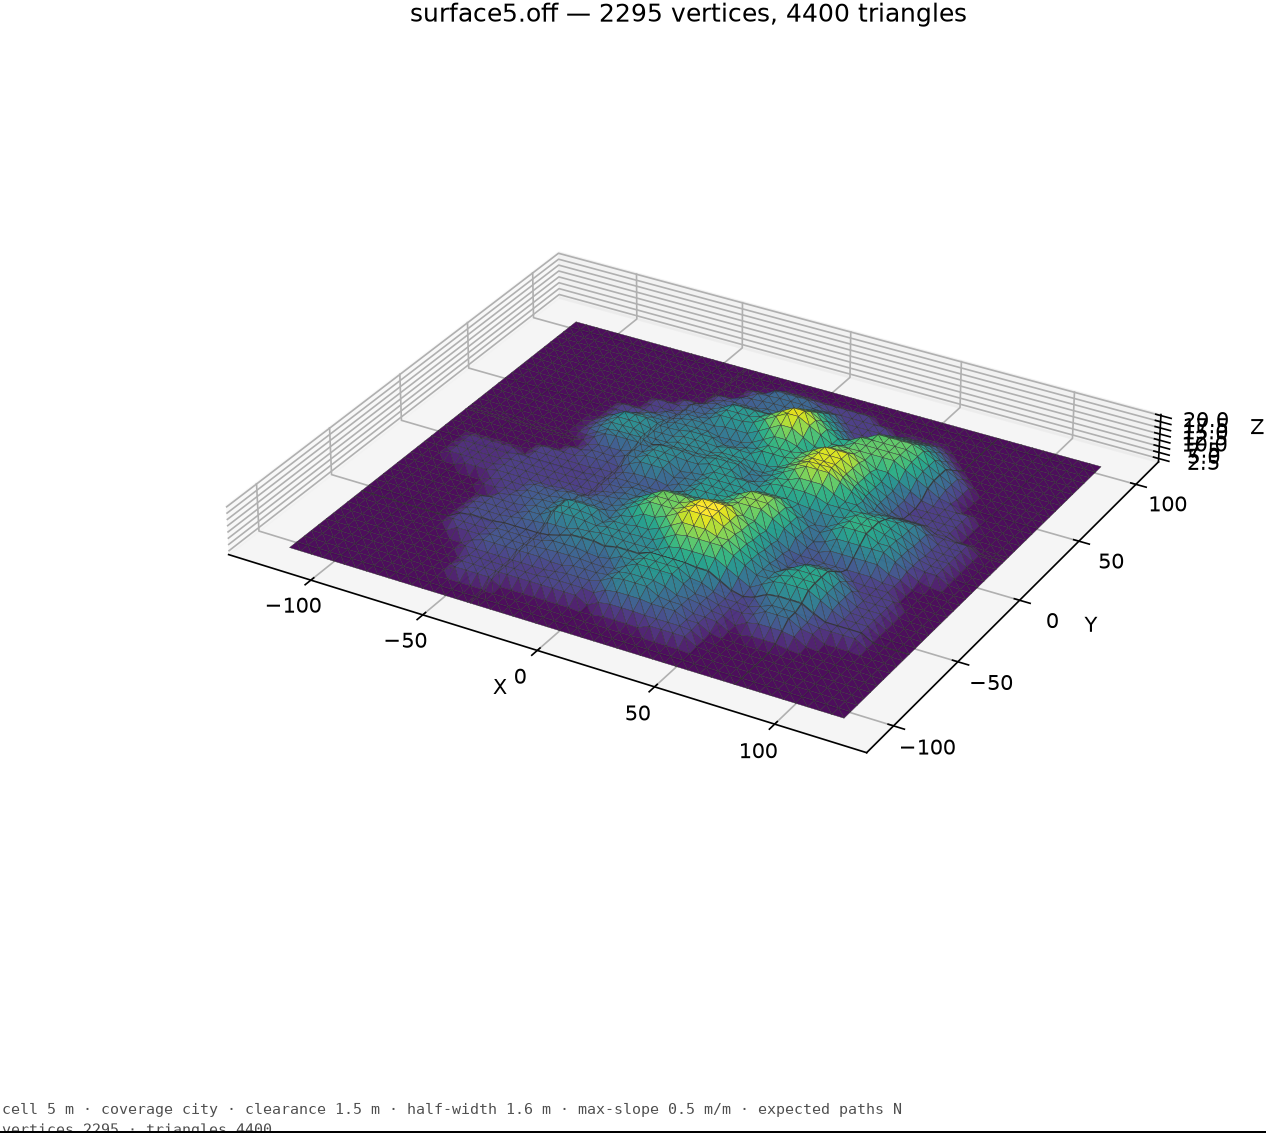
\includegraphics[width=\linewidth]{Figures/crop/repo_surface5.png}
    \caption{Lưới $5$ m: 2\,295 đỉnh, 4\,400 tam giác.}
  \end{subfigure}\par\vspace{2pt}
  \begin{subfigure}{0.60\textwidth}
    \centering
    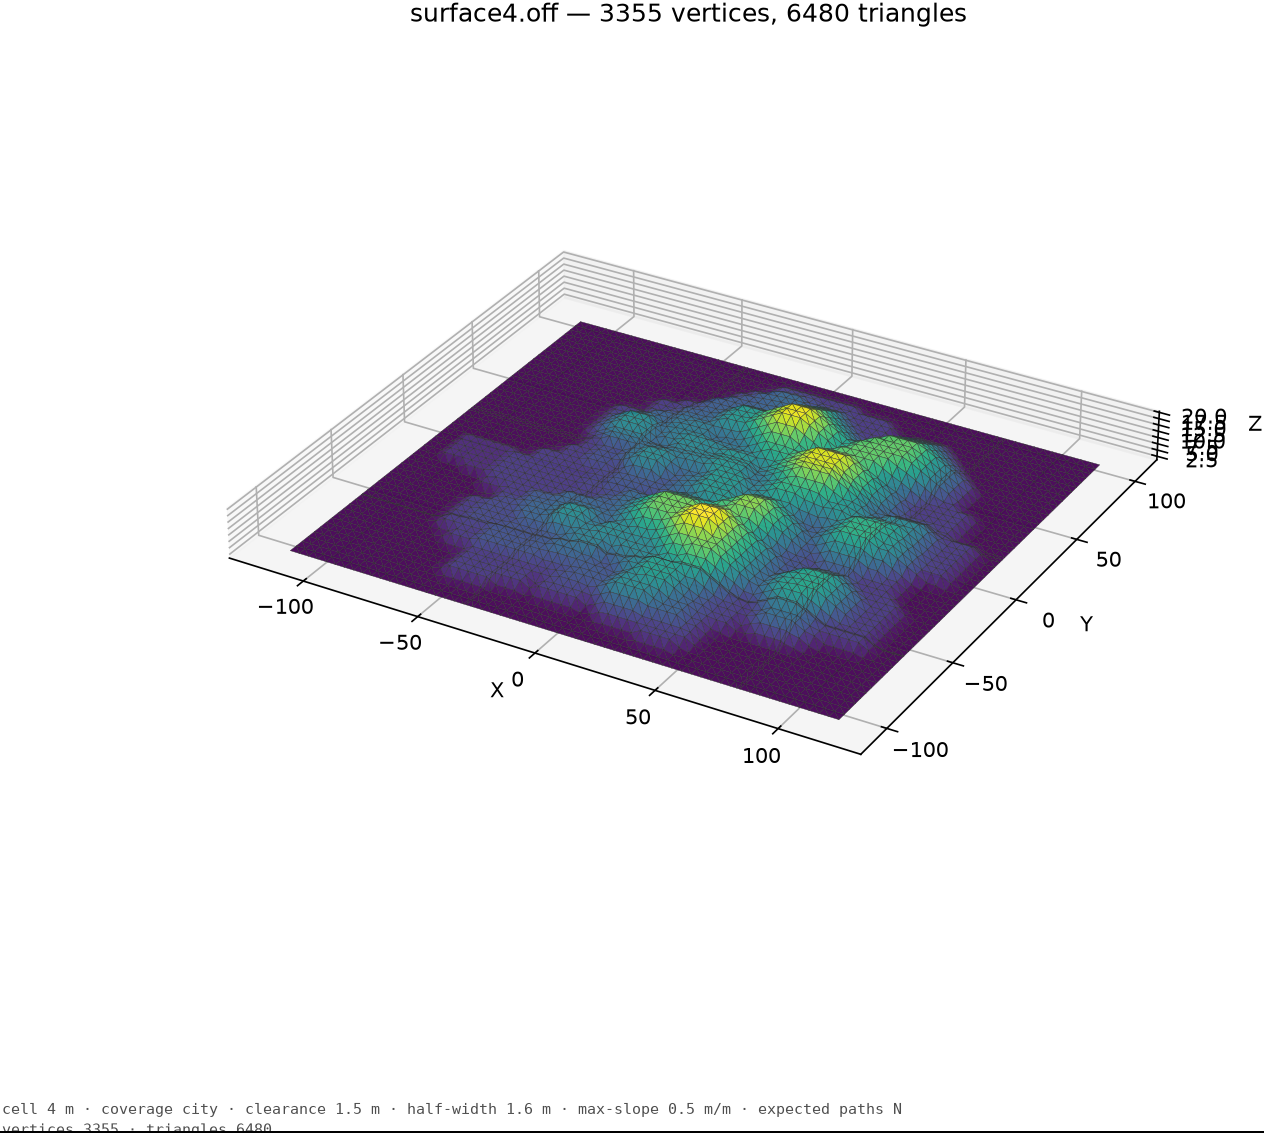
\includegraphics[width=\linewidth]{Figures/crop/repo_surface4.png}
    \caption{Lưới $4$ m: 3\,355 đỉnh, 6\,480 tam giác.}
  \end{subfigure}
  \caption{Hai bề mặt dẫn đường dựng từ cùng một scene, chỉ khác kích thước ô:
    lưới $5$ m (trên) và lưới $4$ m (dưới). Màu là cao độ; các gờ sáng là vùng có
    công trình cao bên dưới.}
  \label{fig:surfaces-54}
\end{figure*}

\begin{figure*}[!t]
  \centering
  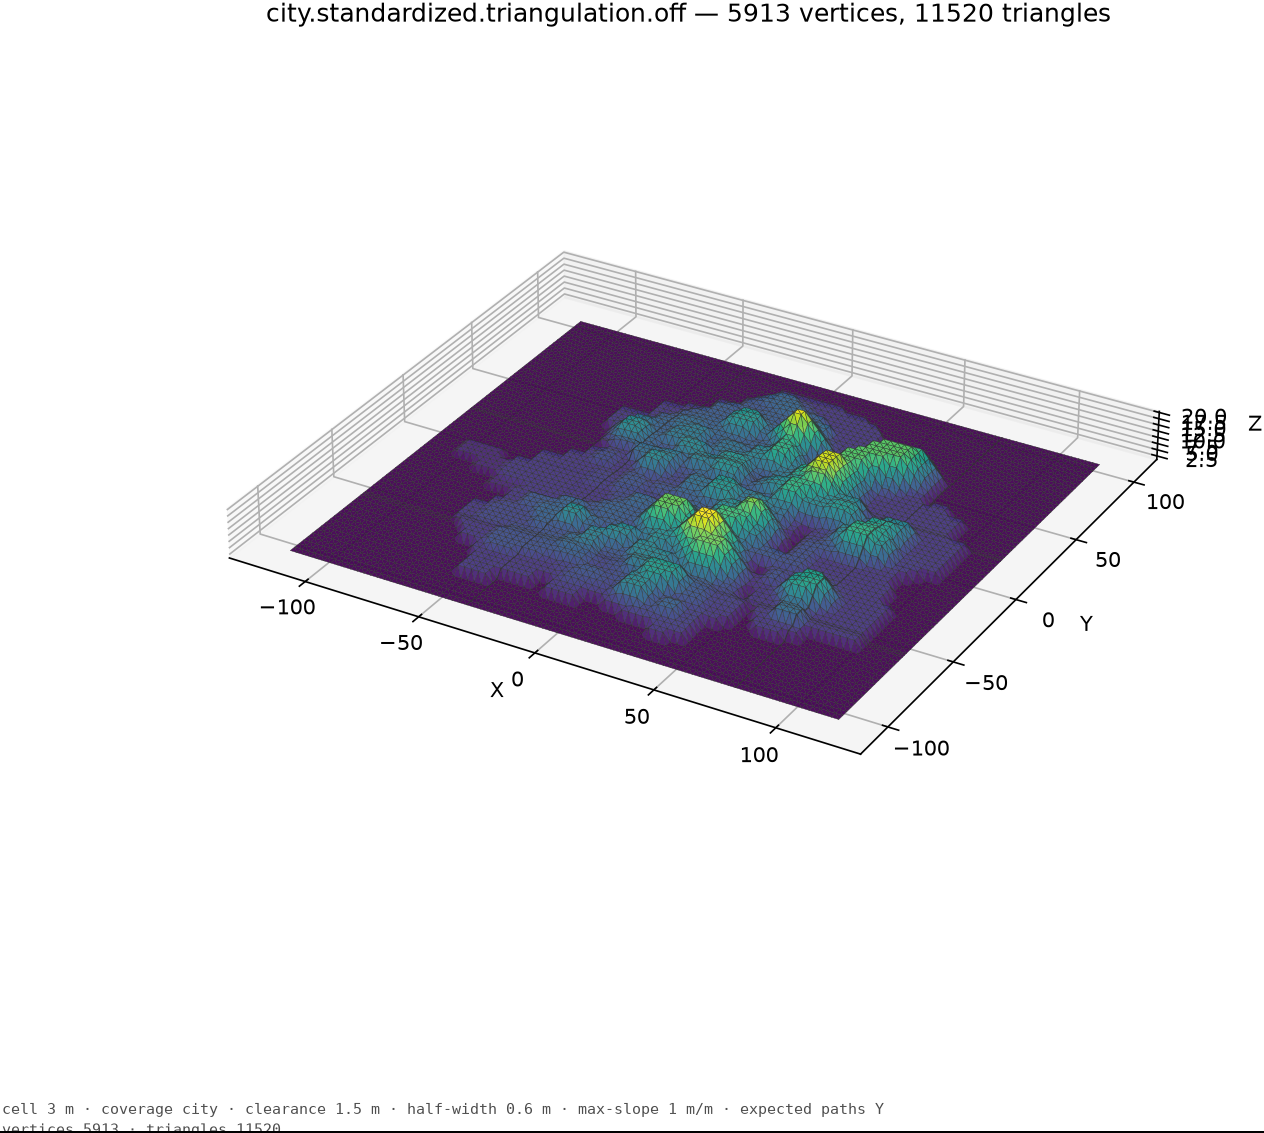
\includegraphics[width=0.75\textwidth]{Figures/crop/repo_surface3.png}
  \caption{Bề mặt dẫn đường lưới $3$ m: 5\,913 đỉnh, 11\,520 tam giác. So với hai
    lưới trên, mật độ tam giác cao hơn và các vách dốc $45^\circ$ rõ hơn.}
  \label{fig:surface-3}
\end{figure*}

Hình~\ref{fig:surfaces-54} và Hình~\ref{fig:surface-3} cho thấy mật độ tam giác
tăng rõ từ lưới $5$ lên lưới $4$ rồi lưới $3$, trong khi hình dạng tổng thể của
envelope vẫn giữ các “dãy” cao độ theo công trình. Lưới $5$ và $4$ dùng cùng dự
phòng ngang và cùng độ dốc, nên khác biệt chủ yếu là độ mịn; lưới $3$ có thêm các
vách dốc $45^\circ$ và bám sát hình học hơn, thể hiện ở các gờ nhọn và vùng
chuyển tiếp hẹp hơn. Đây là hình ảnh định tính tương ứng với các số đo ở
Bảng~\ref{tab:surfaces}.

\begin{figure*}[!t]
  \centering
  \begin{subfigure}{0.62\textwidth}
    \centering
    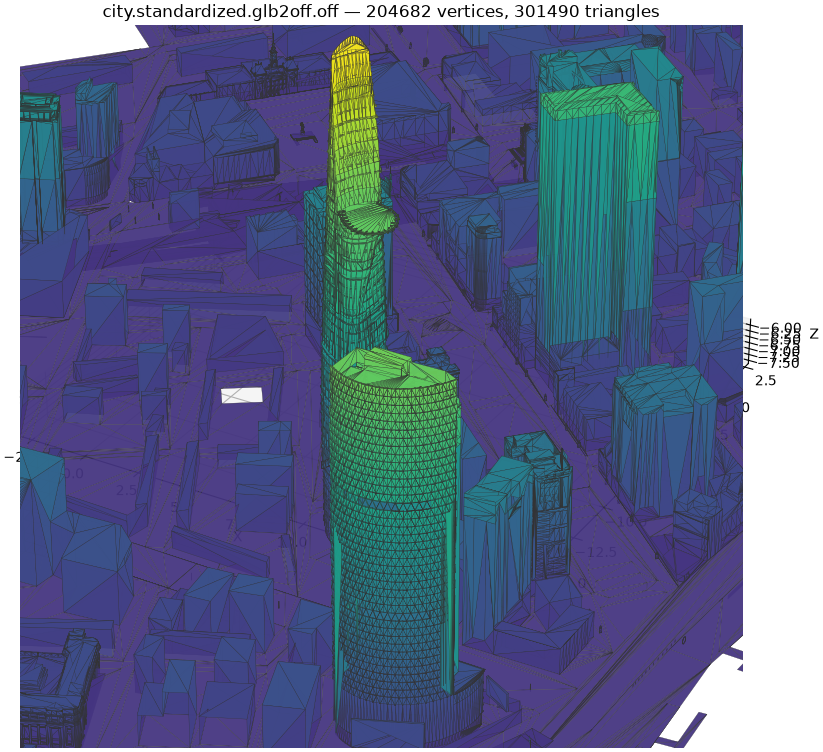
\includegraphics[width=\linewidth]{Figures/crop/etc_city_close.png}
    \caption{Cận cảnh scene: các khối nhà và tháp được tô theo độ cao.}
  \end{subfigure}\par\vspace{2pt}
  \begin{subfigure}{0.62\textwidth}
    \centering
    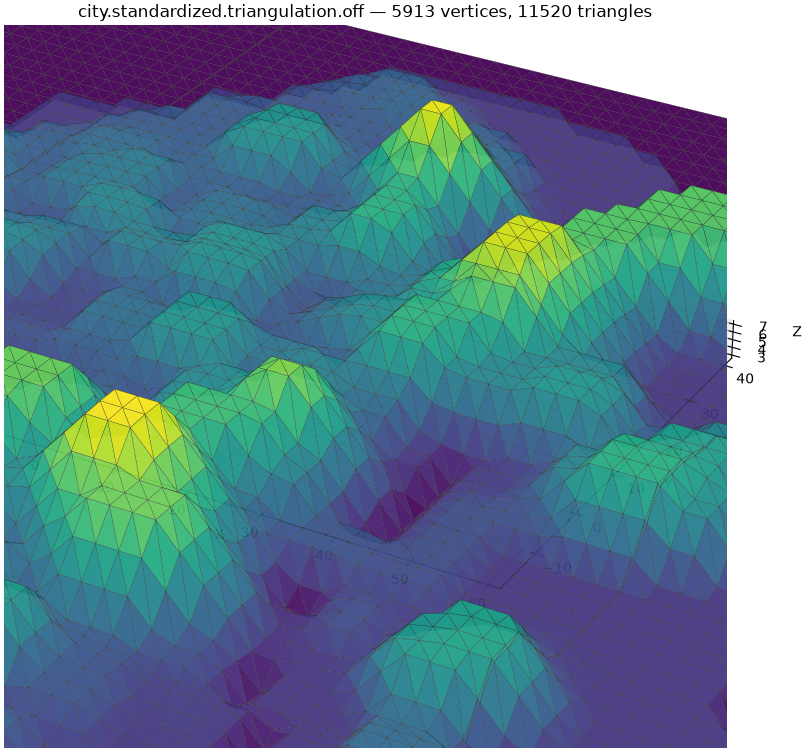
\includegraphics[width=\linewidth]{Figures/crop/etc_surface_close.png}
    \caption{Cận cảnh bề mặt: các tam giác phủ lên công trình và tạo đỉnh/dốc.}
  \end{subfigure}
  \caption{Cận cảnh scene thành phố và bề mặt dẫn đường. Bề mặt không sao chép
    mái nhà; nó nâng lên theo hộp bao công trình rồi hạ dần thành ramp, nên các
    đỉnh tam giác nằm phía trên nóc nhà.}
  \label{fig:city-data}
\end{figure*}

Hình~\ref{fig:city-data} cho thấy rõ hơn quan hệ giữa hai lớp: panel (a) là hình
học công trình với các tháp cao thấp khác nhau; panel (b) là cùng vùng đó nhưng
đã được phủ bởi lưới tam giác của envelope. Các tam giác có kích thước đều theo
ô, nhưng cao độ thay đổi theo công trình bên dưới, tạo ra các “đỉnh” và “yên
ngựa” mà tuyến phải đi qua. Đây là lý do đường đi trên bề mặt không trùng với
đường chim bay và có thể dài hơn khoảng cách Euclid.

\begin{figure*}[!t]
  \centering
  \begin{subfigure}{0.62\textwidth}
    \centering
    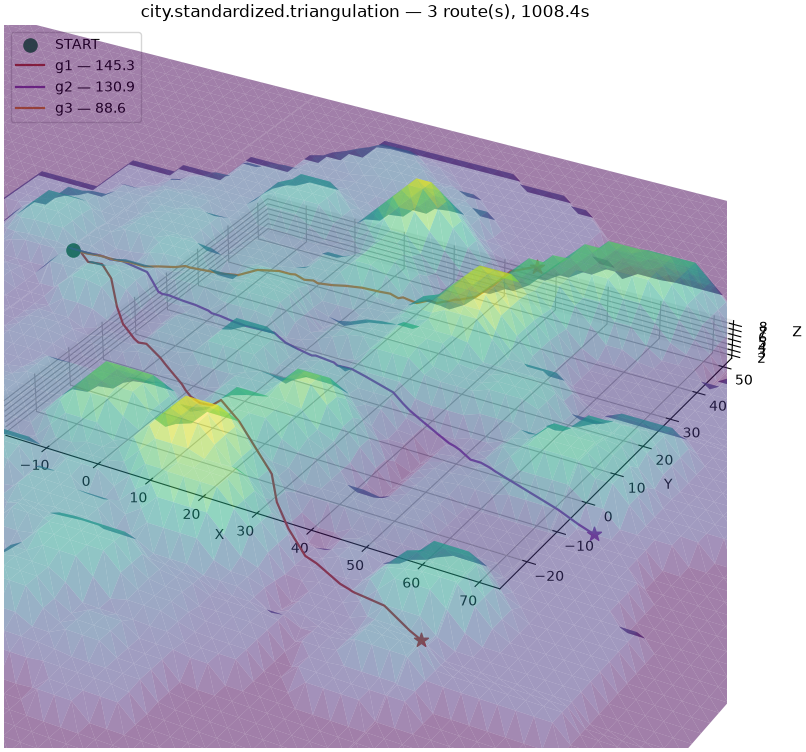
\includegraphics[width=\linewidth]{Figures/crop/etc_routes_3d.png}
    \caption{Góc nhìn 3D: tuyến bám theo các đỉnh và dốc của envelope.}
  \end{subfigure}\par\vspace{2pt}
  \begin{subfigure}{0.62\textwidth}
    \centering
    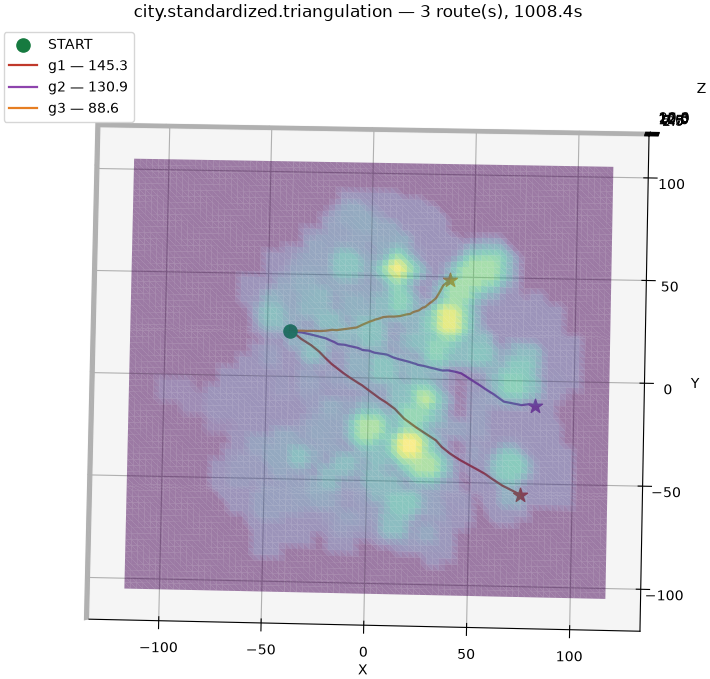
\includegraphics[width=\linewidth]{Figures/crop/etc_routes_top.png}
    \caption{Hình chiếu bằng: ba tuyến từ cùng một nguồn đến ba đích.}
  \end{subfigure}
  \caption{Cận cảnh tuyến trên bề mặt lưới $3$ m. Panel (a) cho thấy độ cao thay
    đổi dọc tuyến; panel (b) cho thấy hình dạng ngang và việc các tuyến tách
    nhau ngay sau nguồn.}
  \label{fig:routes-detail}
\end{figure*}


\subsection{Lập tuyến và đối chiếu tham chiếu}\label{sec:stage-plan}

Funnel Tree chạy trên từng mission. Với mission nhiều goal, mỗi goal được tìm
trong một lượt riêng: một lượt chung giữ frontier theo goal xa nhất và làm số lần
lan truyền tăng mạnh trên bề mặt thành phố, nên chế độ \texttt{per-goal} được
chọn cho phần thành phố. Đánh đổi là ưu thế một nguồn -- mọi đích của thuật toán
không được khai thác trọn vẹn. Trên đồ thị nguồn phụ, thuật toán dùng A* với
heuristic Euclid $h(v)=\norm{v-g}$ (khi tắt heuristic, hàng đợi ưu tiên thoái hóa
thành Dijkstra); mỗi đỉnh được settle một lần rồi lan truyền phễu. Giới hạn thời gian áp cho từng lượt
tìm, giới hạn số nút chặn lan truyền bùng nổ, và Thủ tục 2 được bật.

Mỗi route ghi waypoint 3D, độ dài (tổng Euclid giữa các waypoint), số lần lan
truyền, thời gian từng goal, cùng hash của mission, mesh và mã thuật toán. Nhờ đó
một dòng trong bảng có thể truy ngược về đúng đầu vào sinh ra nó. Bảng~\ref{tab:planning}
trình bày độ dài, số waypoint và chi phí tìm kiếm của ba cấu hình. Độ dài là tổng
khoảng cách giữa các waypoint trên bề mặt, tính trước bước rút gọn Douglas--Peucker
với dung sai $0{,}1$ dùng cho chuyến bay; sau rút gọn, số waypoint mà plugin thực
sự bay là $27/25/24$ (lưới $5$), $27/24/26$ (lưới $4$) và $30/38/33$ (lưới $3$).

\begin{table*}[!t]
  \caption{Độ dài tuyến và chi phí lập tuyến trên ba bề mặt. $L$ tính bằng mét của
    mô hình thu nhỏ; $w$ là số waypoint trước khi rút gọn; $P$ là số lần lan truyền của
    từng goal; $T_{\rm plan}$ là thời gian tường của cả ba lượt tìm.}
  \label{tab:planning}
  {\fontsize{7}{8.6}\selectfont
  \begin{adjustbox}{max width=\textwidth}
  \begin{tabular}{@{}lrrrrrrrrr@{}}
    \toprule
    Cấu hình & $L_{\rm G1}$ & $L_{\rm G2}$ & $L_{\rm G3}$
      & $w_{\rm G1}/w_{\rm G2}/w_{\rm G3}$
      & $P_{\rm G1}$ & $P_{\rm G2}$ & $P_{\rm G3}$ & $\sum P$ & $T_{\rm plan}$ (s) \\
    \midrule
    lưới $5$ & 142,418722 & 125,636333 & 86,152328 & 41/46/40 & 49  & 34  & 21  & 104 & 44,984 \\
    lưới $4$ & 142,909050 & 127,295935 & 86,194146 & 50/59/48 & 81  & 66  & 40  & 187 & 186,175 \\
    lưới $3$ & 145,314559 & 130,891670 & 88,611502 & 65/73/68 & 177 & 150 & 102 & 429 & 1\,008,389 \\
    \bottomrule
  \end{tabular}
  \end{adjustbox}}
\end{table*}

Số lần lan truyền tăng từ $104$ lên $187$ rồi $429$ khi số tam giác tăng từ
$4\,400$ lên $6\,480$ rồi $11\,520$. Thời gian tường tăng nhanh hơn: từ
\num{44.984} giây lên \num{186.175} giây (gấp $4{,}1$ lần) và \num{1008.389}
giây (gấp $5{,}4$ lần so với lưới $4$). Mỗi cấu hình chỉ được đo một lượt trên
máy chưa khống chế tải, nên các tỉ lệ này chỉ là số liệu quan sát, không dùng để
suy ra độ phức tạp tiệm cận.

Độ dài tuyến tăng khi lưới mịn hơn, nhưng mức tăng không đều: G1 từ
\num{142.418722} lên \num{142.909050} rồi \num{145.314559}; G2 từ
\num{125.636333} lên \num{127.295935} rồi \num{130.891670}. Một phần chênh lệch
đến từ bề mặt mịn hơn bám sát khối công trình hơn và tạo nhiều chỗ lượn hơn,
phần khác đến từ điểm đích được snap lại như đã nêu.

Năm mesh nhỏ có đường tham chiếu độc lập; bước đối chiếu chạy Funnel từ đúng đỉnh
nguồn ghi trong tham chiếu, so độ dài từng polyline với dung sai tương đối
$10^{-4}$; không có đỉnh nào vượt dung sai trên tổng 76 đỉnh. Bốn mesh còn lại và bề mặt
thành phố không có tham chiếu độc lập, nên không có bộ giải thứ hai để khẳng định
tối ưu.

Thay vào đó, tuyến thành phố được kiểm tra bằng một cặp cận độc lập trên chính bề
mặt lưới $3$ m (tệp bề mặt có tám ký tự đầu SHA256 là \texttt{9cec5d09}, trùng
dòng lưới $3$ trong Bảng~\ref{tab:surfaces}). Cận dưới là khoảng cách Euclid $d_E=\norm{x_g-x_s}$, vì mọi đường
trên bề mặt không ngắn hơn đoạn thẳng trong không gian. Cận trên $\ell_G$ là độ
dài đường đi ngắn nhất trên đồ thị cạnh của lưới (Dijkstra theo trọng số là độ dài
cạnh); đường này nằm trọn trên bề mặt nên không thể ngắn hơn đường trắc địa. Mọi
độ dài Funnel Tree phải nằm trong khoảng $[d_E,\ell_G]$, và Bảng~\ref{tab:bounds}
cho thấy cả ba tuyến đều thỏa. Đây là điều kiện cần, không phải chứng minh tối ưu:
khoảng cách tới cận trên còn $4{,}6\,\%$, $4{,}9\,\%$ và $22{,}3\,\%$, phản ánh
việc đường trên đồ thị cạnh bị buộc đi qua đỉnh nên vòng xa hơn, đặc biệt ở G3.

\begin{table}[!t]
  \caption{Kiểm tra kẹp độ dài tuyến trên lưới $3$ m. $d_E$ là cận dưới Euclid,
    $L$ là độ dài Funnel Tree, $\ell_G$ là cận trên từ Dijkstra trên đồ thị cạnh;
    đơn vị là mét của mô hình thu nhỏ.}
  \label{tab:bounds}
  {\fontsize{6.5}{8}\selectfont
  \setlength{\tabcolsep}{3pt}%
  \begin{tabular}{@{}lrrrr@{}}
    \toprule
    Goal & $d_E$ & $L$ & $\ell_G$ & $(\ell_G{-}L)/L$ \\
    \midrule
    g1 & 137,409 & 145,314559 & 151,981 & 4,59\,\% \\
    g2 & 124,533 & 130,891670 & 137,266 & 4,87\,\% \\
    g3 &  82,138 &  88,611502 & 108,404 & 22,34\,\% \\
    \bottomrule
  \end{tabular}}
\end{table}

Cặp cận này chỉ chạy được cho lưới $3$ m vì đây là bề mặt được công bố kèm dữ
liệu; hai lưới còn lại chỉ có route và manifest, không có tệp bề mặt đầy đủ trong
bộ kết quả lưu trữ. Hình~\ref{fig:routes-small} minh họa đầu ra của công cụ vẽ tuyến trên
bảy mesh còn lại; cùng với \texttt{icosahedron} và \texttt{J17}, cả chín mesh đều
có ảnh tuyến.

\begin{figure*}[!t]
  \centering
  \begin{subfigure}{0.235\textwidth}
    \centering
    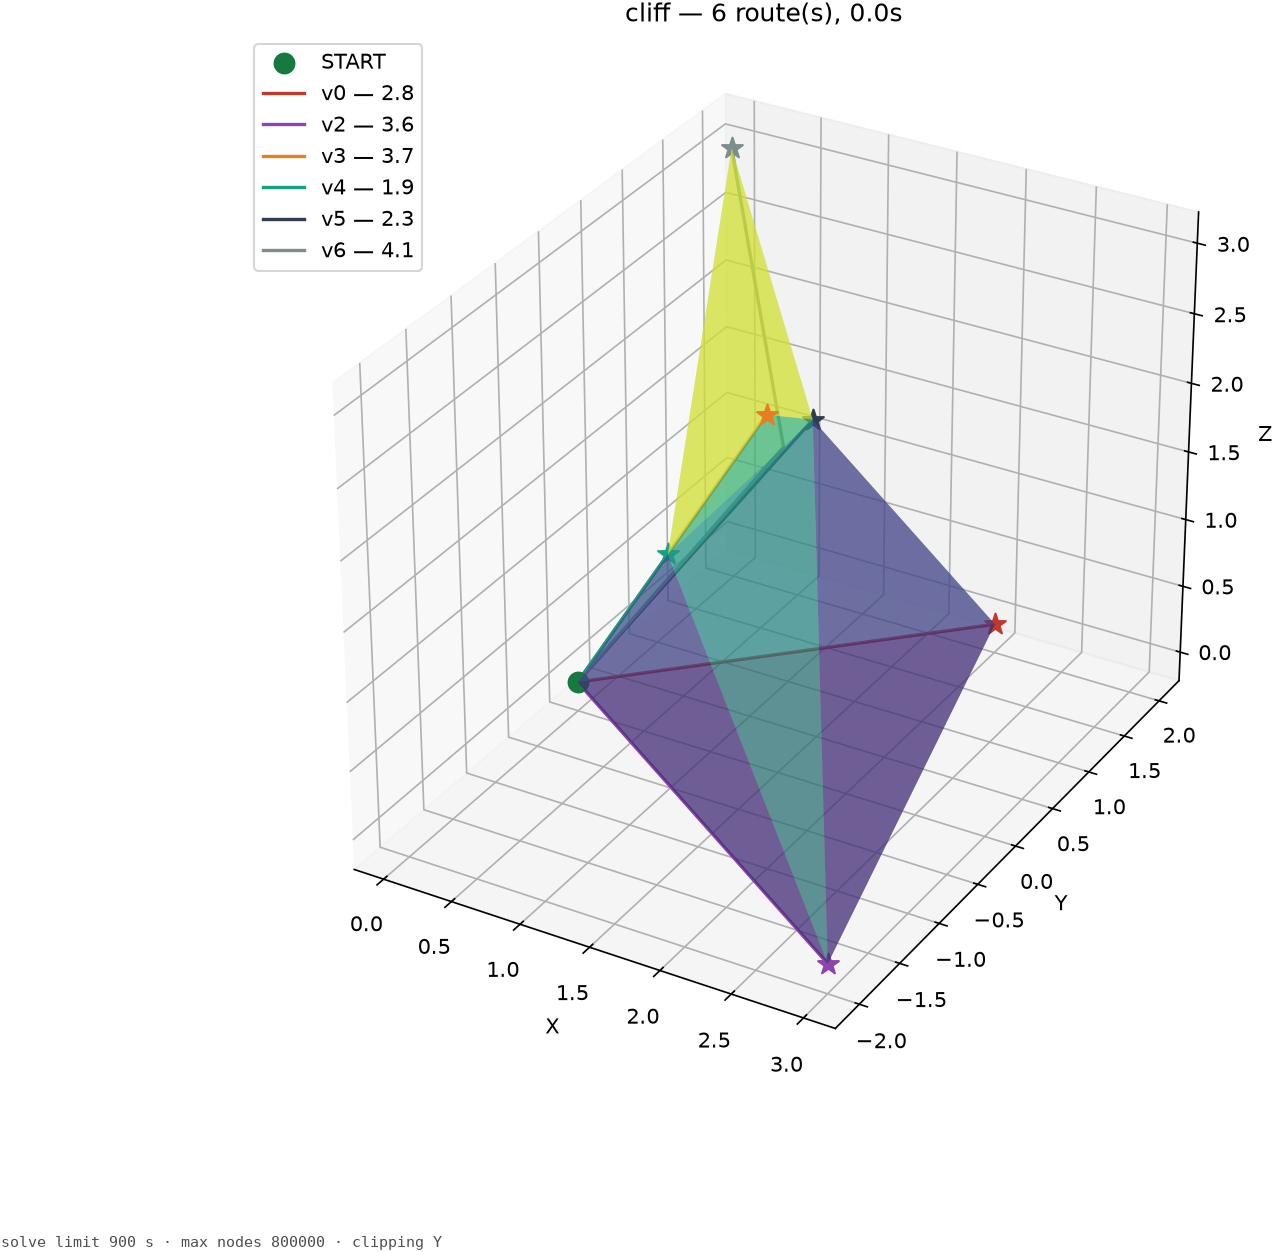
\includegraphics[width=\linewidth]{Figures/crop/repo_cliff_routes.png}
    \caption{\texttt{cliff}}
  \end{subfigure}\hfill
  \begin{subfigure}{0.235\textwidth}
    \centering
    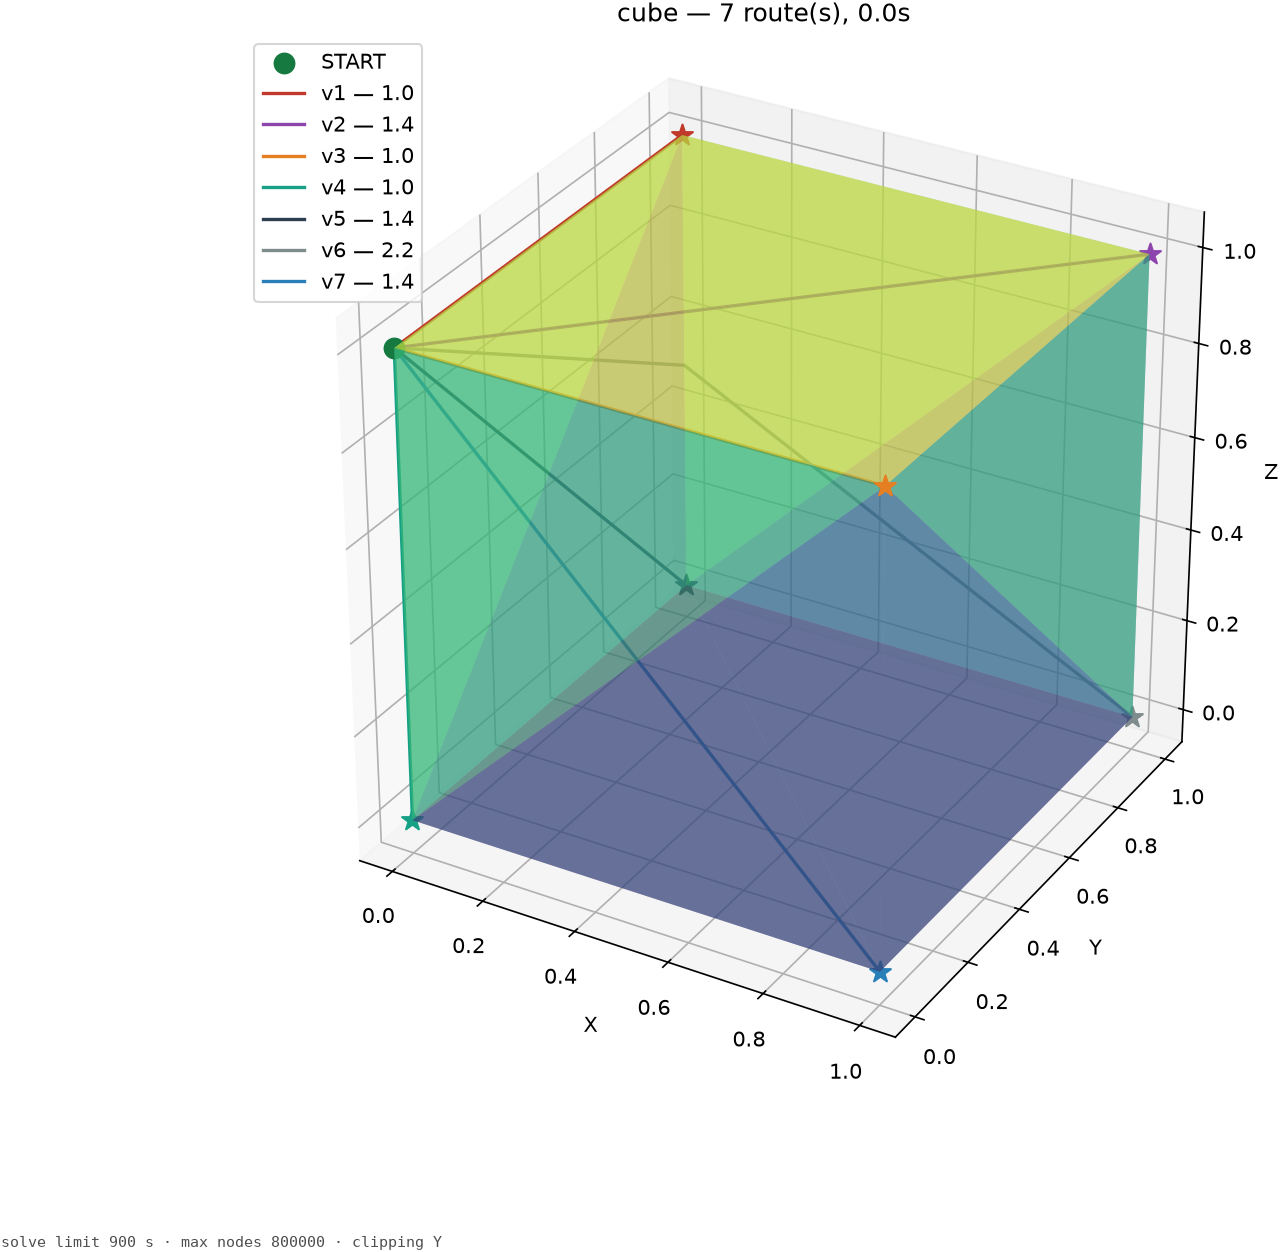
\includegraphics[width=\linewidth]{Figures/crop/repo_cube_routes.png}
    \caption{\texttt{cube}}
  \end{subfigure}\hfill
  \begin{subfigure}{0.235\textwidth}
    \centering
    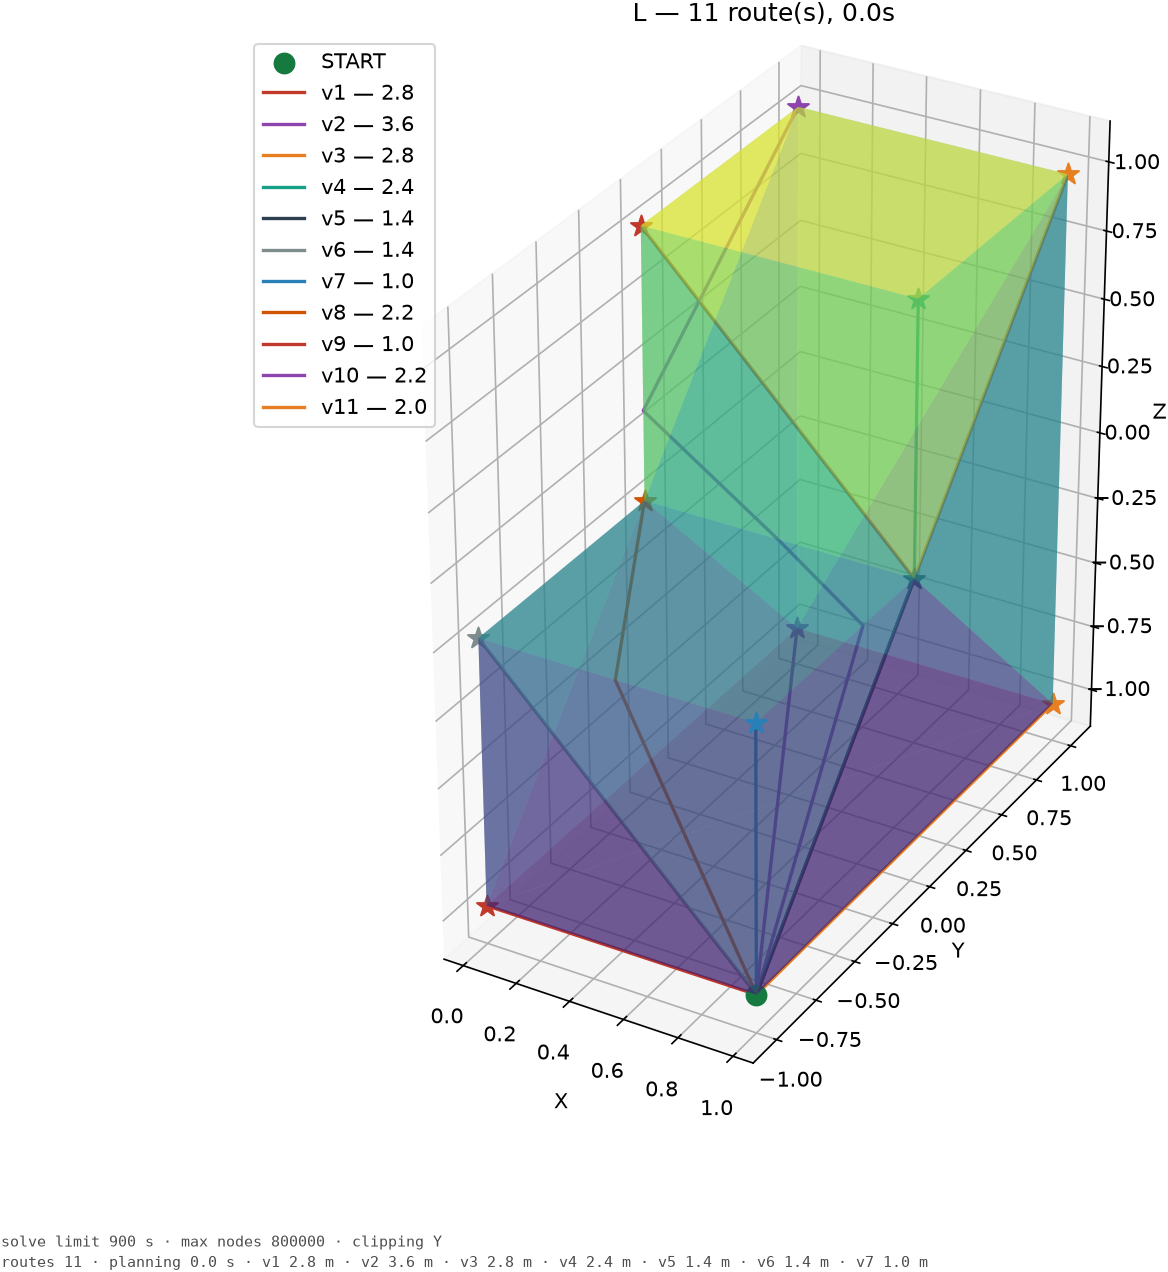
\includegraphics[width=\linewidth]{Figures/crop/repo_L_routes.png}
    \caption{\texttt{L}}
  \end{subfigure}\hfill
  \begin{subfigure}{0.235\textwidth}
    \centering
    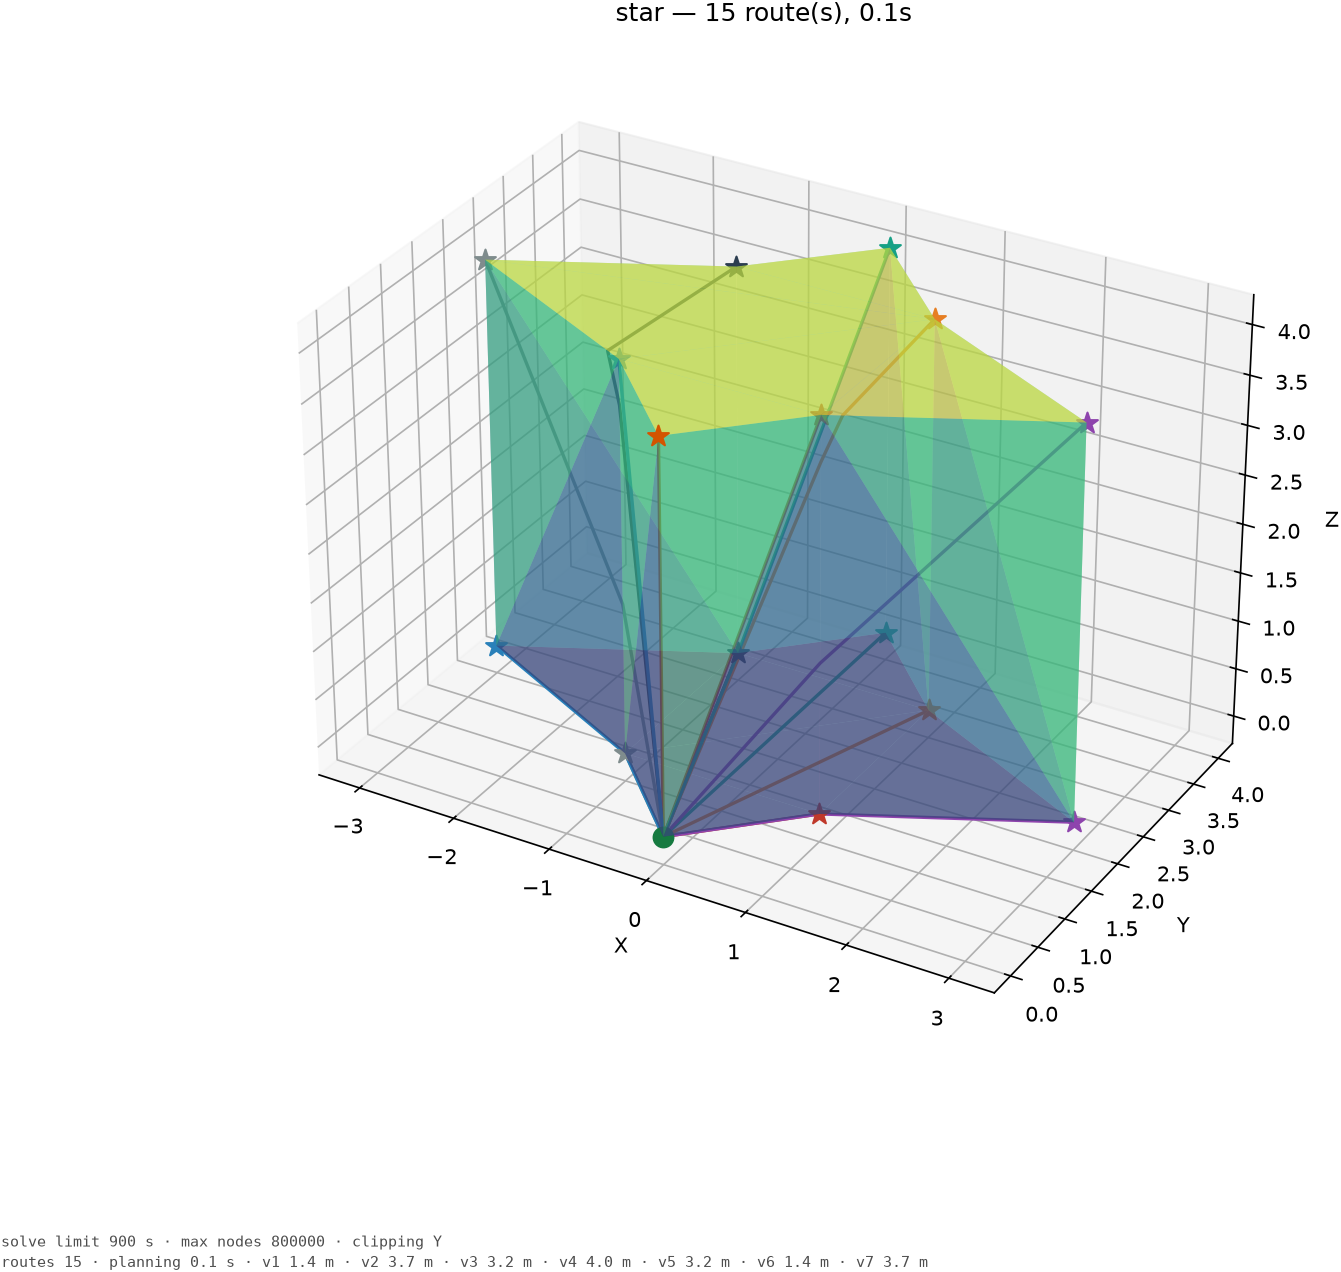
\includegraphics[width=\linewidth]{Figures/crop/repo_star_routes.png}
    \caption{\texttt{star}}
  \end{subfigure}\par\vspace{2pt}
  \hspace*{\fill}%
  \begin{subfigure}{0.235\textwidth}
    \centering
    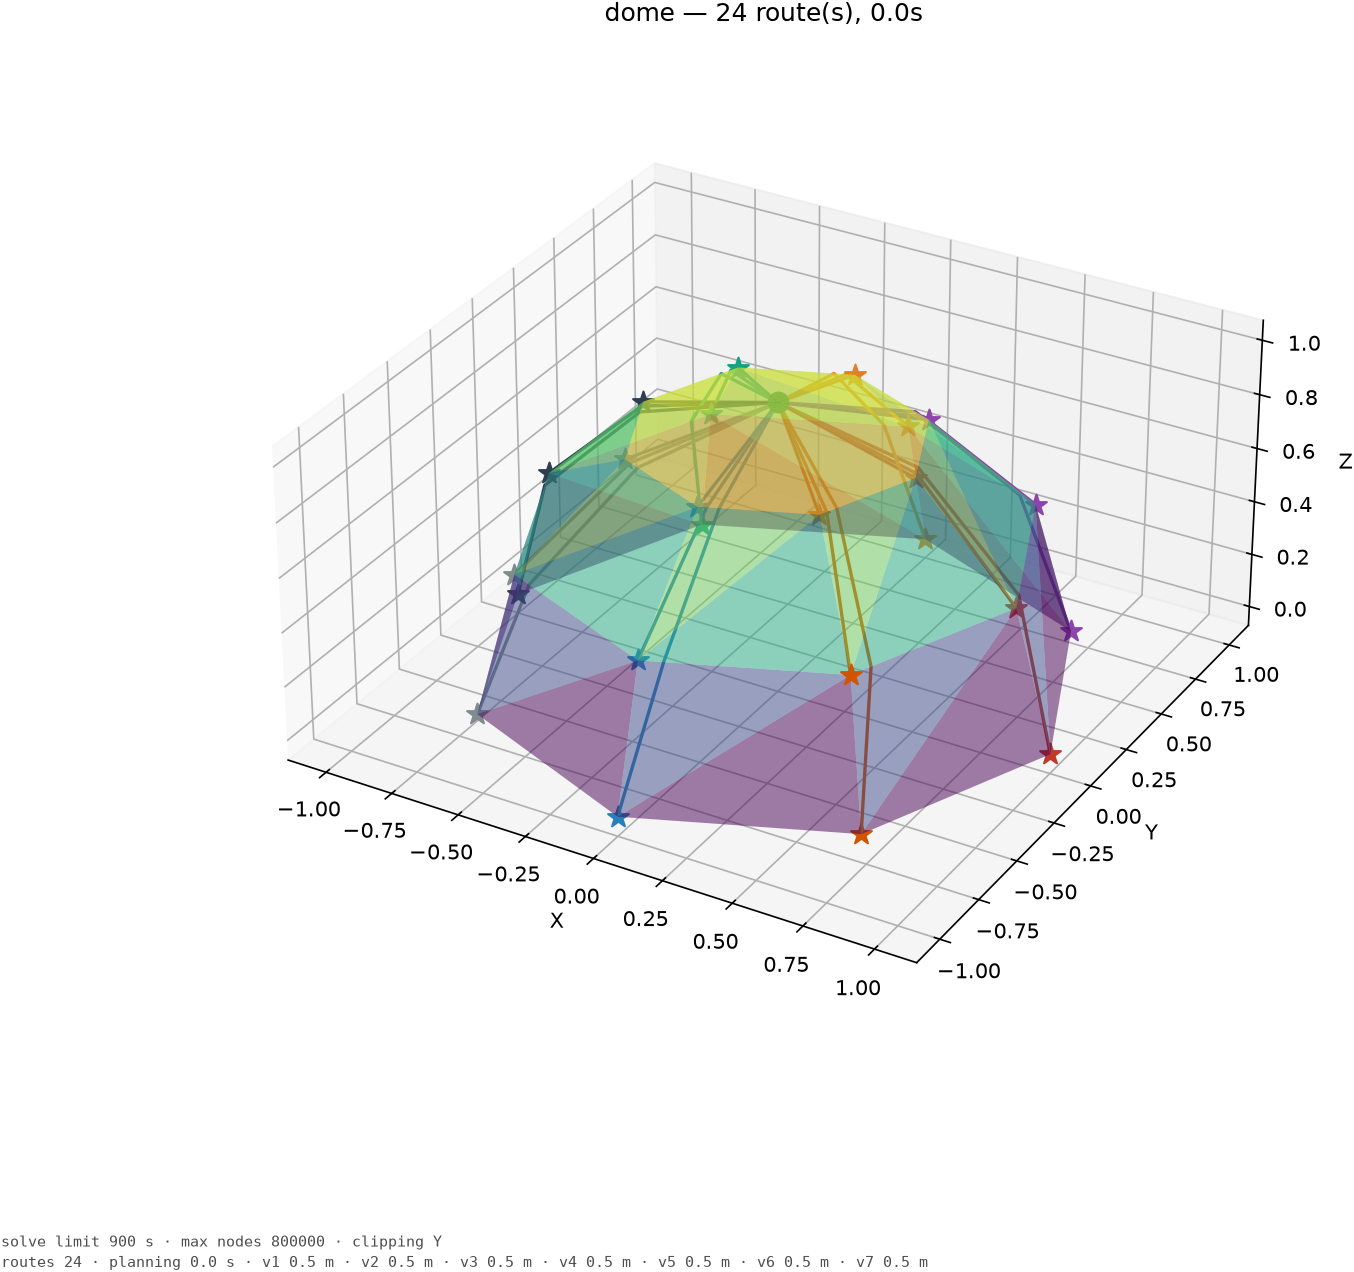
\includegraphics[width=\linewidth]{Figures/crop/repo_dome_routes.png}
    \caption{\texttt{dome}}
  \end{subfigure}\hfill
  \begin{subfigure}{0.235\textwidth}
    \centering
    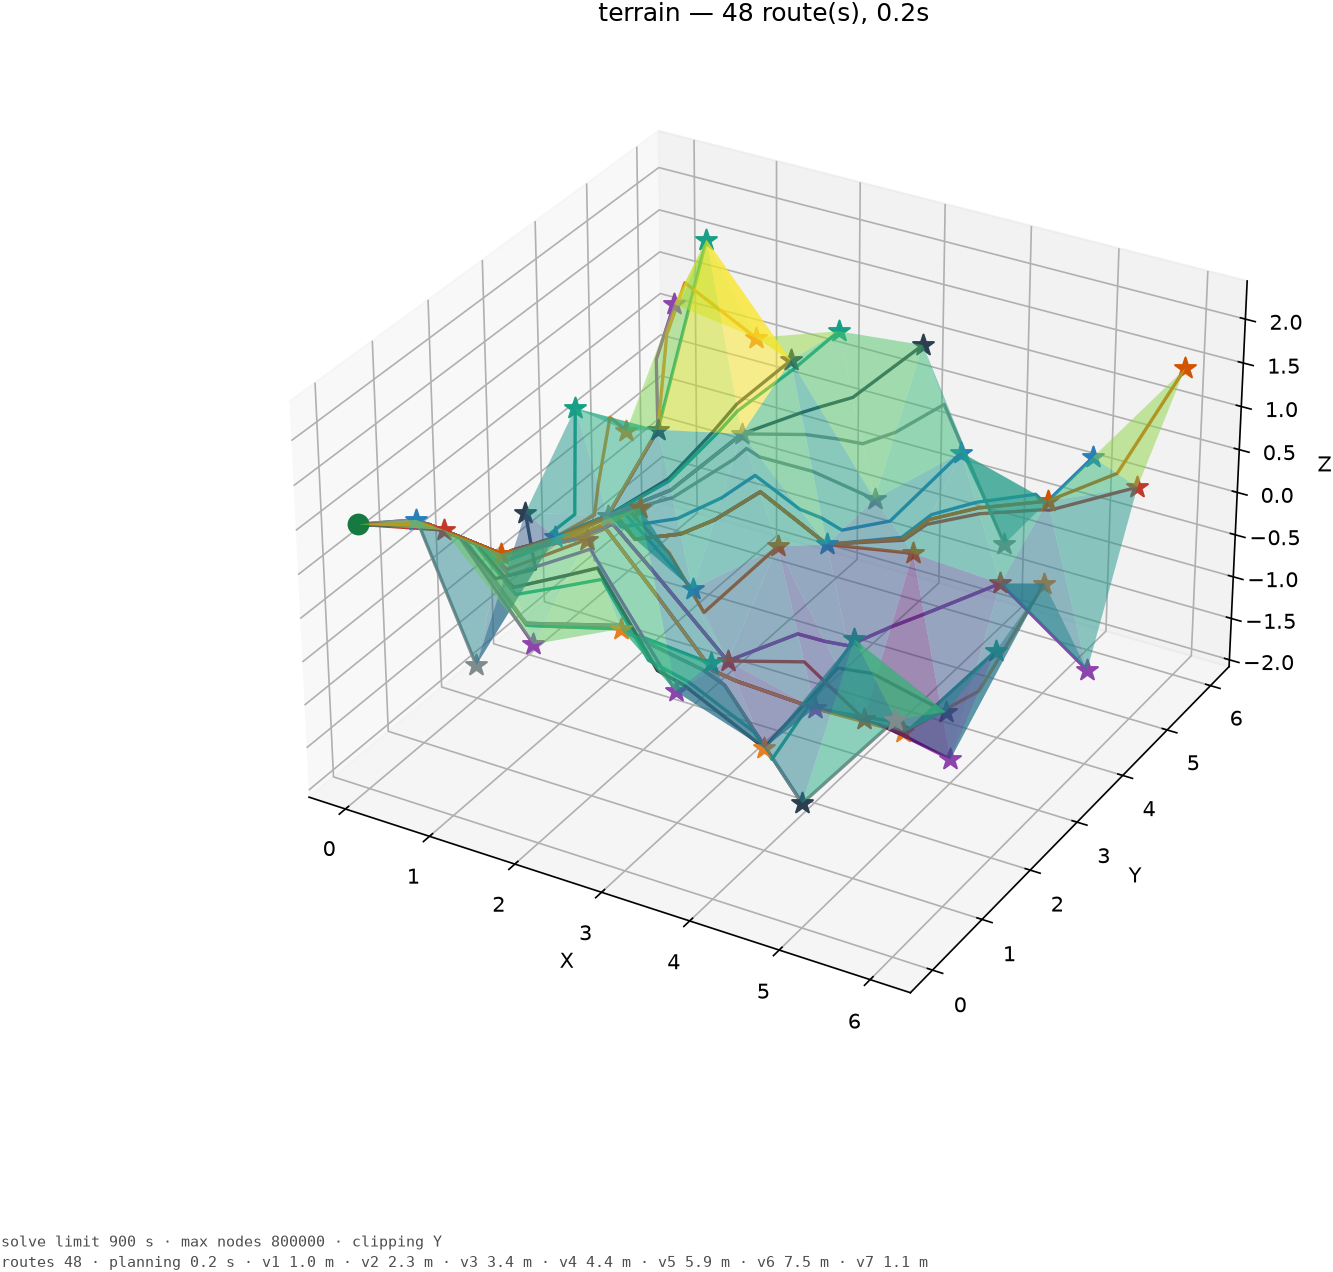
\includegraphics[width=\linewidth]{Figures/crop/repo_terrain_routes.png}
    \caption{\texttt{terrain}}
  \end{subfigure}\hfill
  \begin{subfigure}{0.235\textwidth}
    \centering
    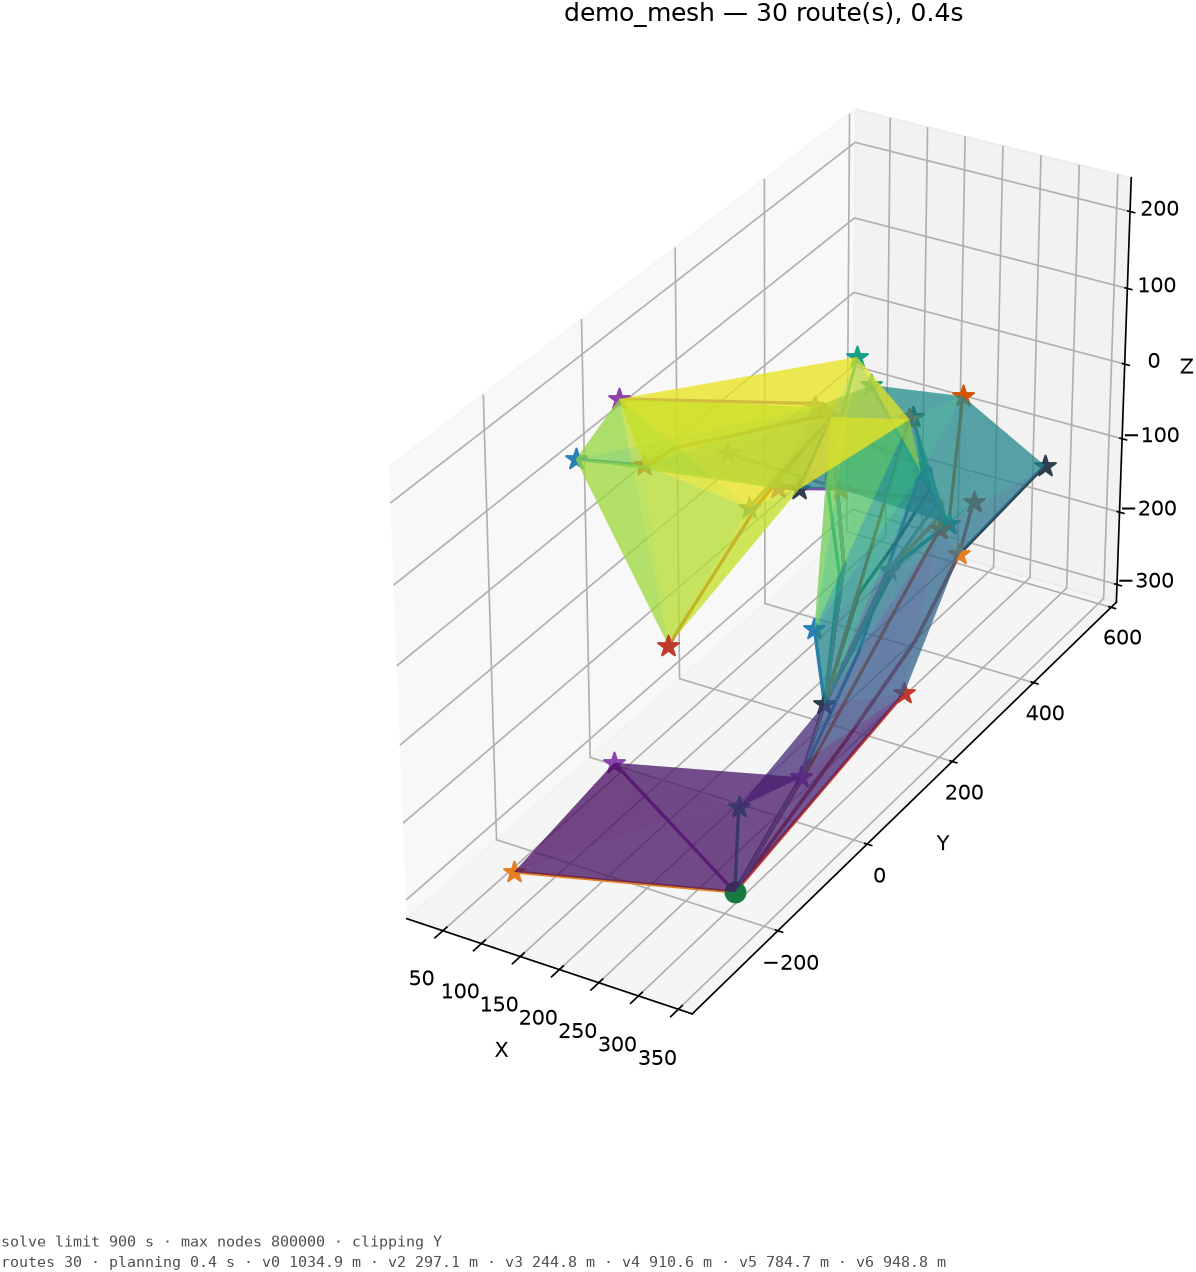
\includegraphics[width=\linewidth]{Figures/crop/repo_demo_mesh_routes.png}
    \caption{\texttt{demo\_mesh}}
  \end{subfigure}%
  \hspace*{\fill}
  \caption{Đầu ra của công cụ vẽ tuyến trên bảy mesh còn lại. Cùng với
    \texttt{icosahedron} và \texttt{J17}, cả chín mesh của bộ dữ liệu đều có ảnh
    tuyến.}
  \label{fig:routes-small}
\end{figure*}

Hình~\ref{fig:routes-small} cho thấy công cụ vẽ tuyến giữ được hình dạng đặc
trưng của từng mesh: \texttt{cliff} có các tuyến gãy qua sườn dốc, \texttt{star}
có các nhánh tỏa theo múi, \texttt{dome} và \texttt{terrain} có tuyến men theo
biên mở, còn \texttt{demo\_mesh} có tuyến vòng qua lỗ xuyến. Đây là kiểm tra định
tính rằng cùng một quy trình lập tuyến chạy được trên bề mặt kín, không lồi và mở;
phần định lượng vẫn là đối chiếu độ dài ở Bảng~\ref{tab:ket-qua-tong-the}.

\subsection{Mô hình UAV, quỹ đạo và telemetry}\label{sec:trajectory}

Đường hình học do Funnel Tree trả về là một polyline trên bề mặt. Để tránh dừng
lại ở mỗi waypoint, quỹ đạo tham chiếu được dựng bằng spline Catmull--Rom đi qua
toàn bộ waypoint. Với các điểm $p_0,\ldots,p_{n-1}$, tiếp tuyến tại $p_i$ là
\begin{equation}
  m_i=
  \begin{cases}
    p_1-p_0, & i=0,\\
    \tfrac12\left(p_{i+1}-p_{i-1}\right), & 0<i<n-1,\\
    p_{n-1}-p_{n-2}, & i=n-1,
  \end{cases}
  \label{eq:tangent}
\end{equation}
và vị trí trên đoạn $p_i\to p_{i+1}$ là
\begin{equation}
  \begin{split}
    q(u)={}&h_{00}(u)\,p_i+h_{10}(u)\,m_i\\
         &+h_{01}(u)\,p_{i+1}+h_{11}(u)\,m_{i+1},
  \end{split}
  \label{eq:catmullrom}
\end{equation}
với $0\le u\le 1$, trong đó $h_{00}=2u^3-3u^2+1$,
$h_{10}=u^3-2u^2+u$, $h_{01}=-2u^3+3u^2$ và $h_{11}=u^3-u^2$. Chính cơ sở
Hermite bảo đảm $q(0)=p_i$ và $q(1)=p_{i+1}$ với mọi cách chọn tiếp tuyến;
\eqref{eq:tangent} chỉ quyết định hình dạng đoạn cong giữa hai đầu. Spline được
lấy mẫu cách khoảng $0{,}2$ đơn vị để tính chiều dài cung; vận tốc và hướng tiếp
tuyến liên tục, và phương tiện chỉ dừng ở điểm cuối.

Trên toàn tuyến, một profile vận tốc thang duy nhất gồm ba pha tăng tốc, chạy đều
và giảm tốc được dùng, với tốc độ lớn nhất $v_{\max}=5$ và gia tốc
$a_{\max}=3$. Nếu chiều dài cung $L$ đủ lớn, thời gian tăng tốc là
$T_r=v_{\max}/a_{\max}$ và quãng đường tăng tốc là
$d_r=v_{\max}^2/(2a_{\max})$; ngược lại profile có dạng tam giác với
$v_{\rm peak}=\sqrt{a_{\max}L}$ và $T=2\sqrt{L/a_{\max}}$. Nhiệm vụ có thời gian
chờ khởi đầu $2$ giây và không có thời gian giữ tại waypoint.

Bộ điều khiển dùng vị trí và vận tốc đo trực tiếp từ trạng thái mô phỏng, với
gia tốc lệnh
\begin{equation}
  a_{\mathrm{cmd}}=a_{\mathrm{ff}}+K_p(q-x)+K_d(\dot q-\dot x),
  \label{eq:control}
\end{equation}
trong đó $a_{\mathrm{ff}}$ là gia tốc bù trước của quỹ đạo, gồm thành phần tiếp
tuyến của profile và thành phần hướng tâm $v^2\,\mathrm{d}T/\mathrm{d}s$ được chặn
trong $[-3,3]$ theo từng trục; $K_p=2{,}5$ và $K_d=3{,}2$; mỗi thành phần của
$a_{\mathrm{cmd}}$ được chặn trong $[-6,6]$. Lực tác dụng tại tâm khối lượng được
tính từ gia tốc lệnh và phần bù trọng lực.

UAV là một vật thể $1$ kg có va chạm thân hộp; cánh quạt chỉ để hiển thị. Mô hình
chưa có điều khiển tư thế, động lực học rotor, cảm biến nhiễu, ước lượng trạng thái
hay autopilot, nên kết quả được diễn giải là kiểm tra bám tuyến của mô hình chịu
lực, không phải xác nhận khả năng bay thực. Telemetry ghi mỗi $0{,}1$ giây trong
khi vật lý chạy $1$ ms; sai số bám tại mẫu $k$ là $e_k=\norm{x_k-q_k}$. Bài báo
cáo sai số lớn nhất $e_{\max}=\max_k e_k$, sai số trung bình $\bar e$ trên toàn bộ
mẫu và sai số cuối $e_{\rm final}$ tại thời điểm kết thúc.

\subsection{Dựng world và chạy Gazebo}\label{sec:stage-simulate}

Mỗi goal có một world riêng. World dùng bản visual của thành phố có normal để
Gazebo tô sáng, một bản collision đã decimate bằng vertex clustering với ô
$1{,}0$, và một SDF đặt bước vật lý $0{,}001$ giây, trọng trường $9{,}8$, vật thể
$1$ kg cùng plugin điều khiển. Scene gốc có \num{301490} tam giác; tám tam giác
diện tích bằng không (sliver) bị loại khi ghi STL nên bản dùng để dựng world còn
\num{301482} tam giác. Từ bản này, collision giảm do decimate xuống \num{26296}
tam giác và từ \num{204682} xuống \num{12402} đỉnh, đủ giữ hình dạng để kiểm tra
độ cao nhưng nhẹ hơn cho vật lý. Tuyến kế hoạch
được vẽ bằng các ống trụ và chấm màu tại waypoint; camera đặt ở phía tây-nam để
khung trọn tuyến.

Trước khi bay, tuyến được rút gọn bằng Douglas--Peucker với dung sai $0{,}1$ và
ghi thành một tệp route riêng cho plugin. Với lưới $4$, G1 đi từ $50$ xuống $27$
waypoint; với lưới $3$, G1 đi từ $65$ xuống $30$. Plugin đọc route này, chạy
Catmull--Rom và profile vận tốc, rồi ghi telemetry cùng metadata của phiên.

Gazebo Jetty 10.5 \cite{gazebo} chạy với engine DART. Chế độ mặc định là container
từ image \texttt{ghcr.io/openrobotics/gazebo:jetty-full} (khoảng 3 GB), ghim bằng
digest; chế độ \texttt{--native} dùng Gazebo cài trên máy. Chạy headless thì không
mở GUI và tự dừng khi telemetry có \texttt{phase=complete}; chạy GUI cần X11 và
một backend render. Vật lý chạy trên CPU nên số đo bám tuyến không phụ thuộc GPU.
Bảng~\ref{tab:environment} ghi cấu hình máy và phiên bản dùng khi đo.

\begin{table*}[!t]
  \caption{Môi trường chạy của quy trình. Phiên bản trong image là phiên bản dùng
    khi bay; host dùng để chạy các bước dữ liệu và lập tuyến nếu không dùng
    container.}
  \label{tab:environment}
  {\fontsize{7}{8.6}\selectfont
  \begin{adjustbox}{max width=\textwidth}
  \begin{tabular}{@{}lp{300pt}@{}}
    \toprule
    Thành phần & Giá trị \\
    \midrule
    Host & NixOS 26.11; Intel Core i7-9850H (6 nhân/12 luồng); 15 GiB RAM;
      NVIDIA GeForce MX150; Docker 29.9.1 \\
    Python & 3.14.8 trên host; 3.12.3 trong image \\
    Thư viện & NumPy 2.5.4; Shapely 2.2.0; Matplotlib 3.11.2; Pillow 13.0.0 \\
    Gazebo & Jetty 10.5.0, engine DART, bước vật lý $1$ ms, hệ Z-up \\
    Image nền & \texttt{ghcr.io/openrobotics/gazebo@sha256:452ff649...08c7},
      khoảng 3 GB \\
    Image dự án & \texttt{uav-funnel-tree:pipeline}, dựng từ \texttt{Dockerfile} \\
    Compose & \texttt{pipeline} (NVIDIA qua CDI), \texttt{pipeline-intel}
      (/dev/dri), \texttt{pipeline-software} (llvmpipe) \\
    Runtime & \texttt{FUNNEL\_RUNTIME=native}, \texttt{FUNNEL\_PYTHON=/usr/bin/python3},
      có GUI hoặc headless \\
    \bottomrule
  \end{tabular}
  \end{adjustbox}}
\end{table*}

\subsection{Kết quả bám tuyến}\label{sec:stage-validate}

Một chuyến bay \emph{hợp lệ} nếu pha cuối là \texttt{complete} và
$e_{\rm final}\le\num{0.5}$; chuyến bay \emph{đạt mốc chất lượng} nếu ngoài ra
$e_{\max}\le\num{1.0}$. Hai tiêu chí tách riêng để một góc cua trễ không làm dừng
quy trình, nhưng vẫn được ghi nhận là trượt mốc. Đây là các ngưỡng kỹ thuật đặt
trước cho mô hình thu nhỏ, không suy ra từ dự phòng ngang $r$ hay khoảng hở đứng
$\delta$, và không phải bảo đảm an toàn va chạm.

Chín chuyến bay (ba cấu hình $\times$ ba đích) đều hợp lệ. Bảy chuyến đạt mốc;
hai chuyến trượt mốc đều ở G2, một ở lưới $5$ và một ở lưới $3$. Riêng lưới $4$
đạt mốc ở cả ba đích, với sai số lớn nhất $0{,}399$; $0{,}591$ và $0{,}601$.
Bảng~\ref{tab:tracking} tập hợp các chỉ số từ telemetry đã lưu.

\begin{table*}[!t]
  \caption{Kết quả bám tuyến của chín chuyến bay. $T$ là thời gian mô phỏng,
    $e_{\max}$ và $\bar e$ là sai số lớn nhất và trung bình, $e_{\rm final}$ là
    sai số cuối, $v_{\max}$ là vận tốc đo lớn nhất. Đơn vị là mét của mô hình thu
    nhỏ.}
  \label{tab:tracking}
  {\fontsize{7}{8.6}\selectfont
  \begin{adjustbox}{max width=\textwidth}
  \begin{tabular}{@{}llrrrrrrl@{}}
    \toprule
    Cấu hình & Goal & $T$ (s) & $e_{\max}$ & $\bar e$ & $e_{\rm final}$
      & $v_{\max}$ & Hợp lệ & Đạt mốc \\
    \midrule
    lưới $5$ & g1 & 35,859 & 0,3650 & 0,0666 & 0,0004 & 5,1027 & Có & Đạt \\
             & g2 & 33,143 & 1,0224 & 0,1105 & 0,0000 & 5,0411 & Có & Trượt \\
             & g3 & 24,997 & 0,8517 & 0,0893 & 0,0006 & 5,1533 & Có & Đạt \\
    \midrule
    lưới $4$ & g1 & 35,865 & 0,3994 & 0,0589 & 0,0000 & 5,1272 & Có & Đạt \\
             & g2 & 33,247 & 0,5910 & 0,0633 & 0,0000 & 5,1077 & Có & Đạt \\
             & g3 & 25,096 & 0,6009 & 0,1356 & 0,0013 & 5,0965 & Có & Đạt \\
    \midrule
    lưới $3$ & g1 & 36,466 & 0,5075 & 0,0627 & 0,0001 & 5,1764 & Có & Đạt \\
             & g2 & 33,447 & 1,3808 & 0,1349 & 0,0014 & 5,1646 & Có & Trượt \\
             & g3 & 24,995 & 0,5796 & 0,0906 & 0,0005 & 5,1204 & Có & Đạt \\
    \bottomrule
  \end{tabular}
  \end{adjustbox}}
\end{table*}

Sai số trung bình nằm trong khoảng $0{,}059$--$0{,}136$ và sai số cuối không vượt
$0{,}0014$, cho thấy phương tiện bám quỹ đạo trong phần lớn hành trình và dừng
đúng đích; sai số lớn nhất tập trung ở các góc cua. Vận tốc đo lớn nhất nằm trong
khoảng $5{,}04$--$5{,}18$, hơi vượt giới hạn tham chiếu $5$ do độ vọt lố của bộ
điều khiển và do telemetry lấy mẫu $0{,}1$ giây. Gia tốc đo theo hiệu hữu hạn của
vận tốc đạt tới $9{,}87$; giá trị này không phải giới hạn $3$ của profile tham
chiếu, mà phản ánh các đỉnh hiệu chỉnh của PD tại góc cua, nên không được so trực
tiếp với $a_{\max}$.

Cơ chế trượt mốc ở G2 khác nhau giữa các cấu hình; Bảng~\ref{tab:waypoints} ghi
khoảng cách waypoint và tỉ lệ tiếp tuyến trên đúng tuyến đã rút gọn mà plugin
bay. Với lưới $5$, tuyến còn $25$ waypoint (từ $46$ trước rút gọn) với khoảng
cách không đều; tại một chỗ nối, tiếp tuyến Catmull--Rom dài gấp $7{,}6$ lần đoạn
ngắn kề nó, làm quỹ đạo lùi lại và sai số đạt $1{,}022$ tại góc cua. Với lưới
$4$, tuyến còn $24$ waypoint (từ $59$) đều hơn, tỉ lệ tiếp tuyến giảm còn $3{,}15$
và sai số lớn nhất còn $0{,}591$. Với lưới $3$, tuyến còn $38$ waypoint (từ $73$)
nhưng bề mặt dùng vách dốc $45^\circ$: lúc $7{,}89$ giây, đích leo với vận tốc
đứng $2{,}08$ trong khi vận tốc đứng của phương tiện còn $-0{,}53$; đến
$8{,}19$ giây, phương tiện ở cao độ $5{,}74$ trong khi đích đã lên $7{,}12$ và sai
số đạt $1{,}381$. Bảng~\ref{tab:g2vertical} phân rã sai số tại các mốc này: thành phần đứng chiếm hơn $99\,\%$. Vận tốc đứng tham chiếu
đổi từ $-3{,}57$ m/s sang $+2{,}08$ m/s trong khoảng
$0{,}6$ giây, tương ứng với mức biến thiên trung bình khoảng
$9{,}4$ m/s$^2$. Giá trị này mô tả sự thay đổi vận tốc theo
phương thẳng đứng, trong khi tham số $3$ m/s$^2$ của profile
giới hạn gia tốc tiếp tuyến; hai đại lượng không đồng nhất.
Với cấu hình vận tốc tham chiếu tối đa $5$ m/s và gia tốc
tiếp tuyến tối đa $3$ m/s$^2$, sai số ở ca này chủ yếu theo
phương thẳng đứng tại vùng chuyển tiếp cao độ.
Các hướng cần thử nghiệm gồm giảm tốc độ, làm mượt cao độ
tham chiếu hoặc giảm độ dốc $\lambda$.

G1 và G3 đều đạt mốc ở cả ba cấu hình. Với G1, sai số lớn nhất là $0{,}365$
(lưới $5$), $0{,}399$ (lưới $4$) và $0{,}508$ (lưới $3$); tuyến có $27$ waypoint
trên lưới $5$ và $4$ (Bảng~\ref{tab:waypoints}), tỉ lệ tiếp tuyến lớn nhất
$2{,}92$--$3{,}36$, nên sai số chỉ tăng ở các góc cua và vẫn dưới mốc. Với G3, sai số lớn nhất là $0{,}852$ (lưới
$5$), $0{,}601$ (lưới $4$) và $0{,}580$ (lưới $3$); lưới $4$ có trung bình cao
nhất ($0{,}136$) vì tuyến có $26$ waypoint với đoạn ngắn nhất $0{,}777$ và tỉ lệ
tiếp tuyến $5{,}40$, nhưng sai số lớn nhất vẫn dưới $1$. Hai ví dụ này cho thấy
tỉ lệ tiếp tuyến chỉ giải thích được một phần sai số: lưới $5$ ở G3 có tỉ lệ
$1{,}65$ nhưng sai số $0{,}852$, cao hơn lưới $4$ ở G1 ($2{,}92$ và $0{,}399$),
nên độ dốc cao độ và mật độ điểm cũng đóng góp đáng kể.

\begin{figure*}[!t]
  \centering
  \begin{subfigure}{0.66\textwidth}
    \centering
    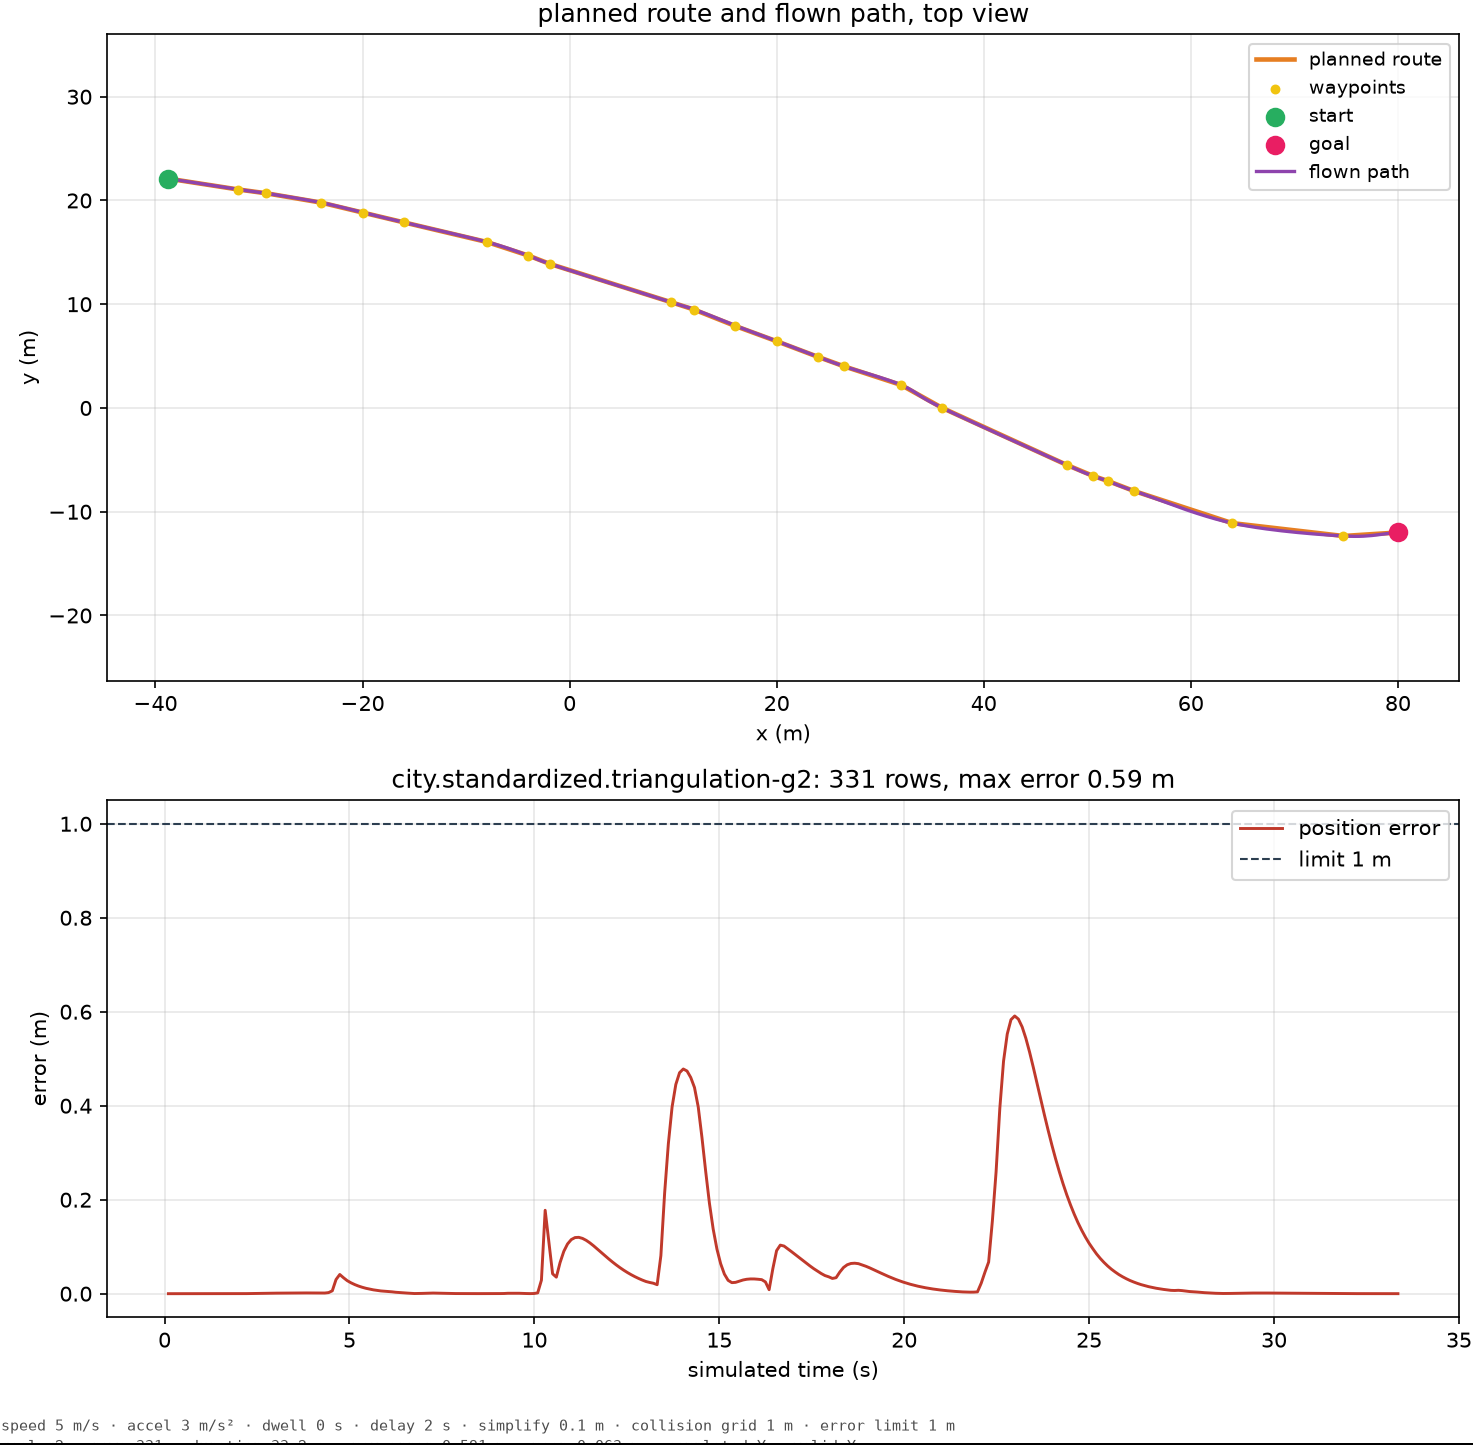
\includegraphics[width=\linewidth]{Figures/crop/cell4_g2_tracking.png}
    \caption{Lưới $4$, G2: $e_{\max}=0{,}591$, đạt mốc.}
  \end{subfigure}\par\vspace{2pt}
  \begin{subfigure}{0.66\textwidth}
    \centering
    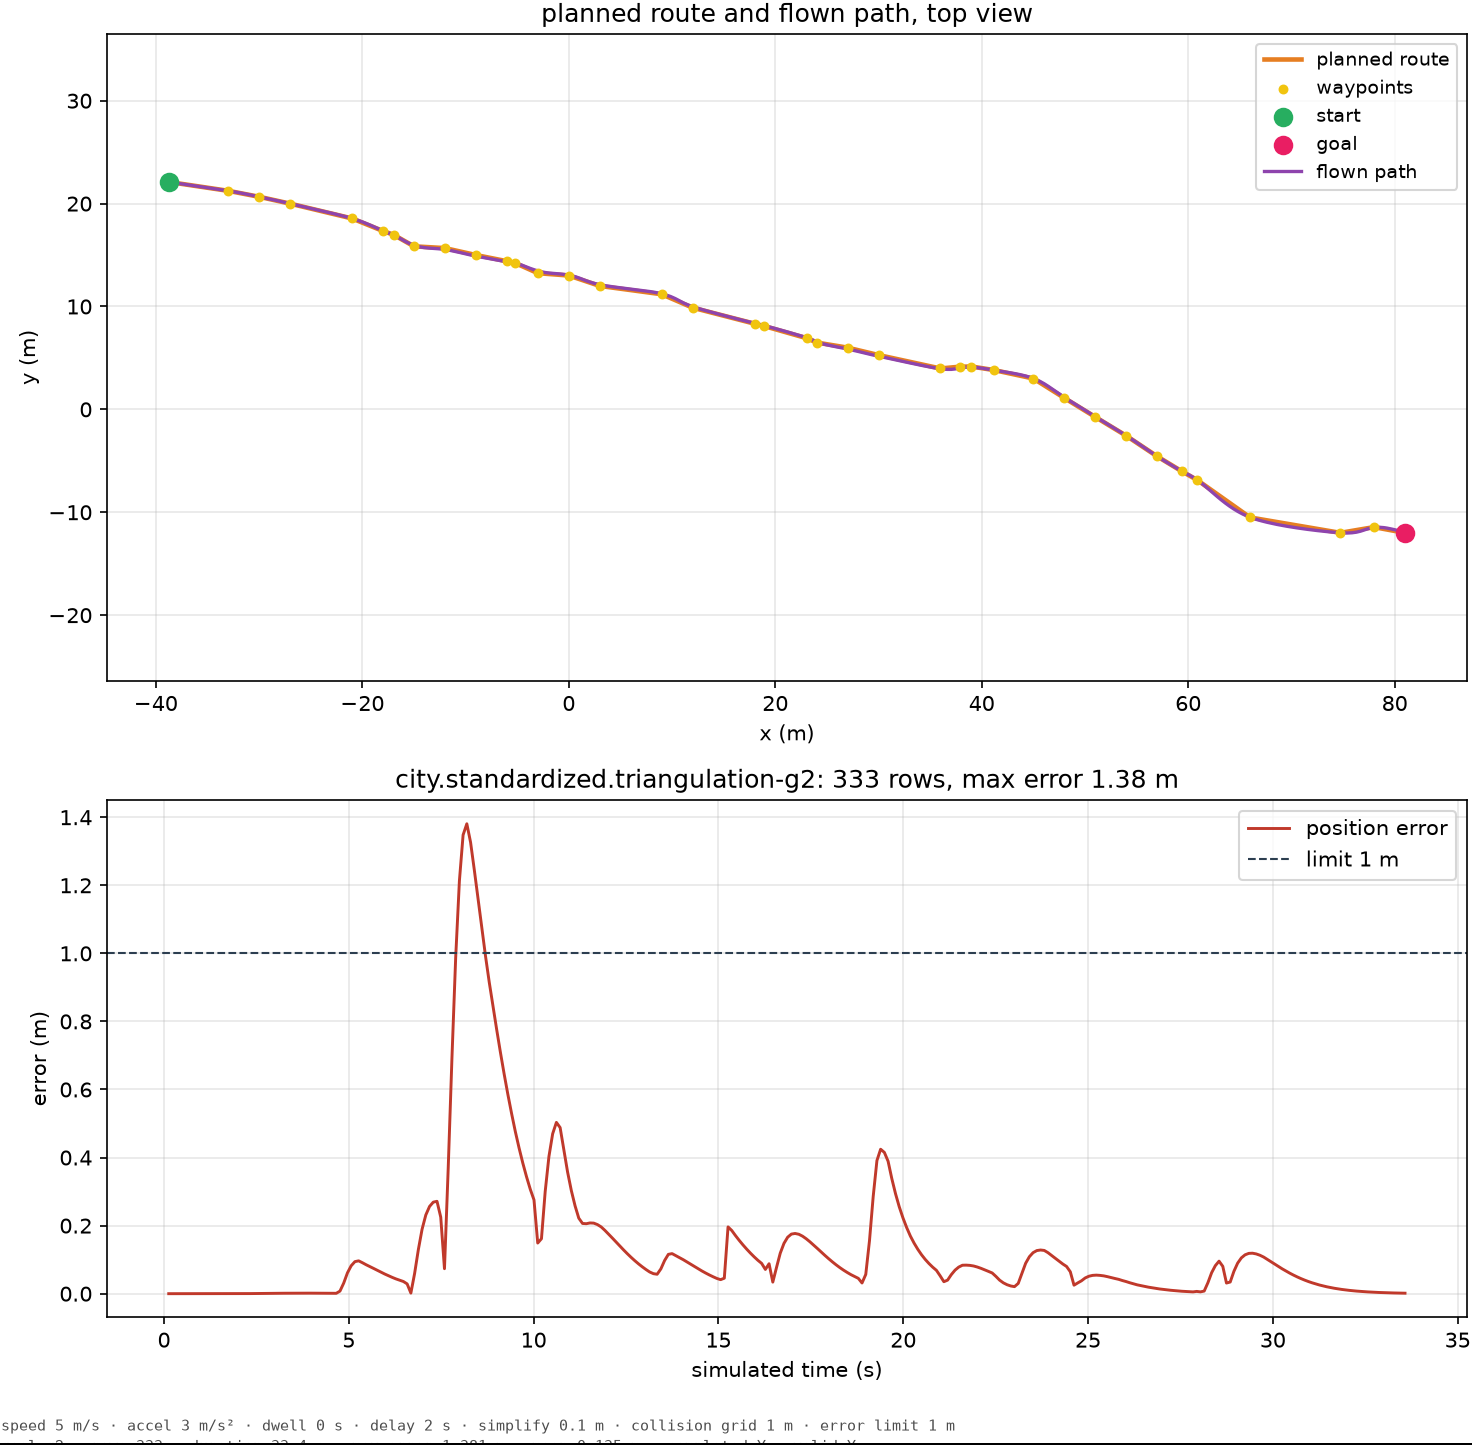
\includegraphics[width=\linewidth]{Figures/crop/cell3_g2_tracking.png}
    \caption{Lưới $3$, G2: $e_{\max}=1{,}381$, trượt mốc do sai số thẳng đứng.}
  \end{subfigure}
  \caption{Đường đã bay và sai số theo thời gian ở đích G2. Panel trên là mặt
    bằng tuyến kế hoạch (cam) và đường đã bay (tím); panel dưới là sai số, nét
    đứt là mốc $1$ đơn vị.}
  \label{fig:tracking}
\end{figure*}

Hình~\ref{fig:tracking} cho thấy đường bay gần như phủ lên tuyến kế hoạch ở
panel mặt bằng; khác biệt nằm ở panel sai số, nơi các đỉnh xuất hiện đúng tại các
góc cua. Với lưới $4$, đỉnh lớn nhất $0{,}591$ vẫn dưới mốc; với lưới $3$, đỉnh
$1{,}381$ vượt mốc và tập trung trong khoảng $7$--$9$ giây, đúng giai đoạn leo
vách dốc.

\begin{figure*}[!t]
  \centering
  \begin{subfigure}{0.66\textwidth}
    \centering
    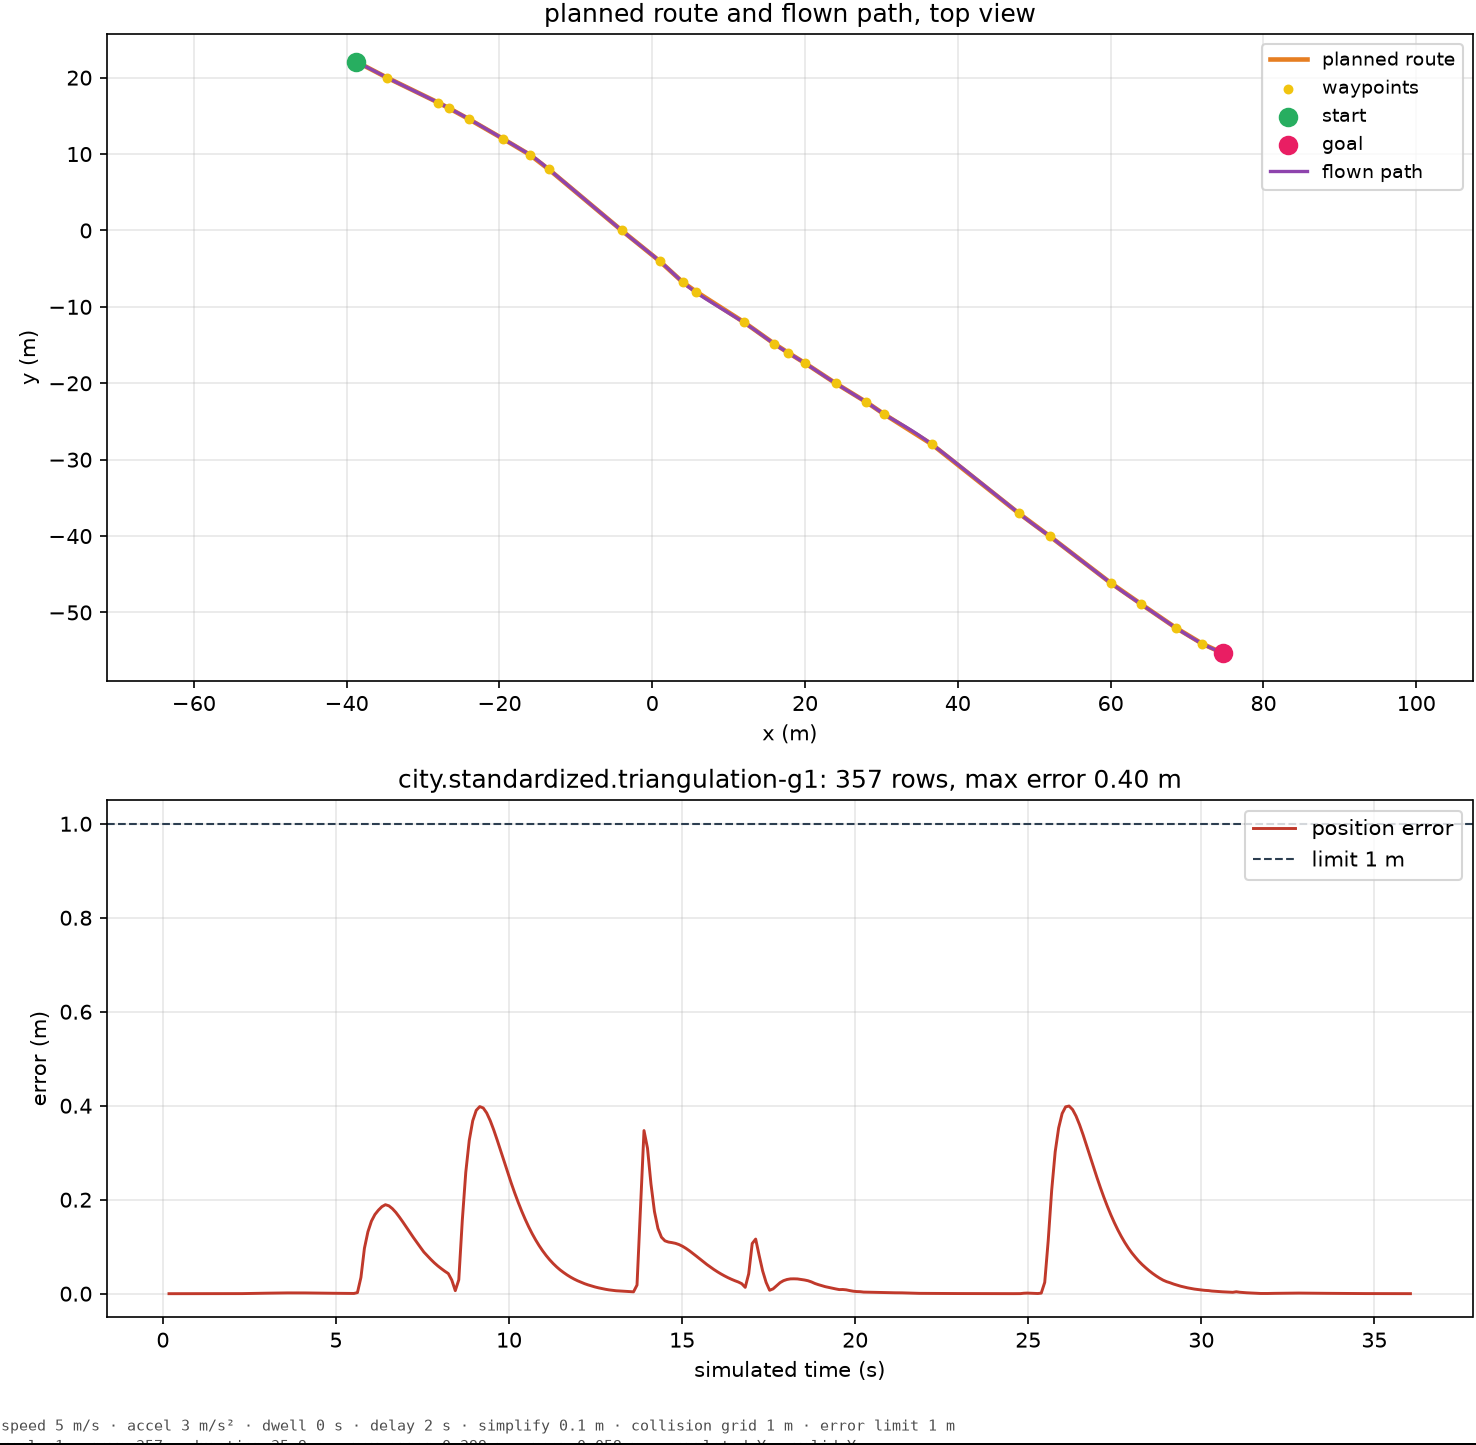
\includegraphics[width=\linewidth]{Figures/crop/cell4_g1_tracking.png}
    \caption{Lưới $4$, G1: $e_{\max}=0{,}399$, đạt mốc.}
  \end{subfigure}\par\vspace{2pt}
  \begin{subfigure}{0.66\textwidth}
    \centering
    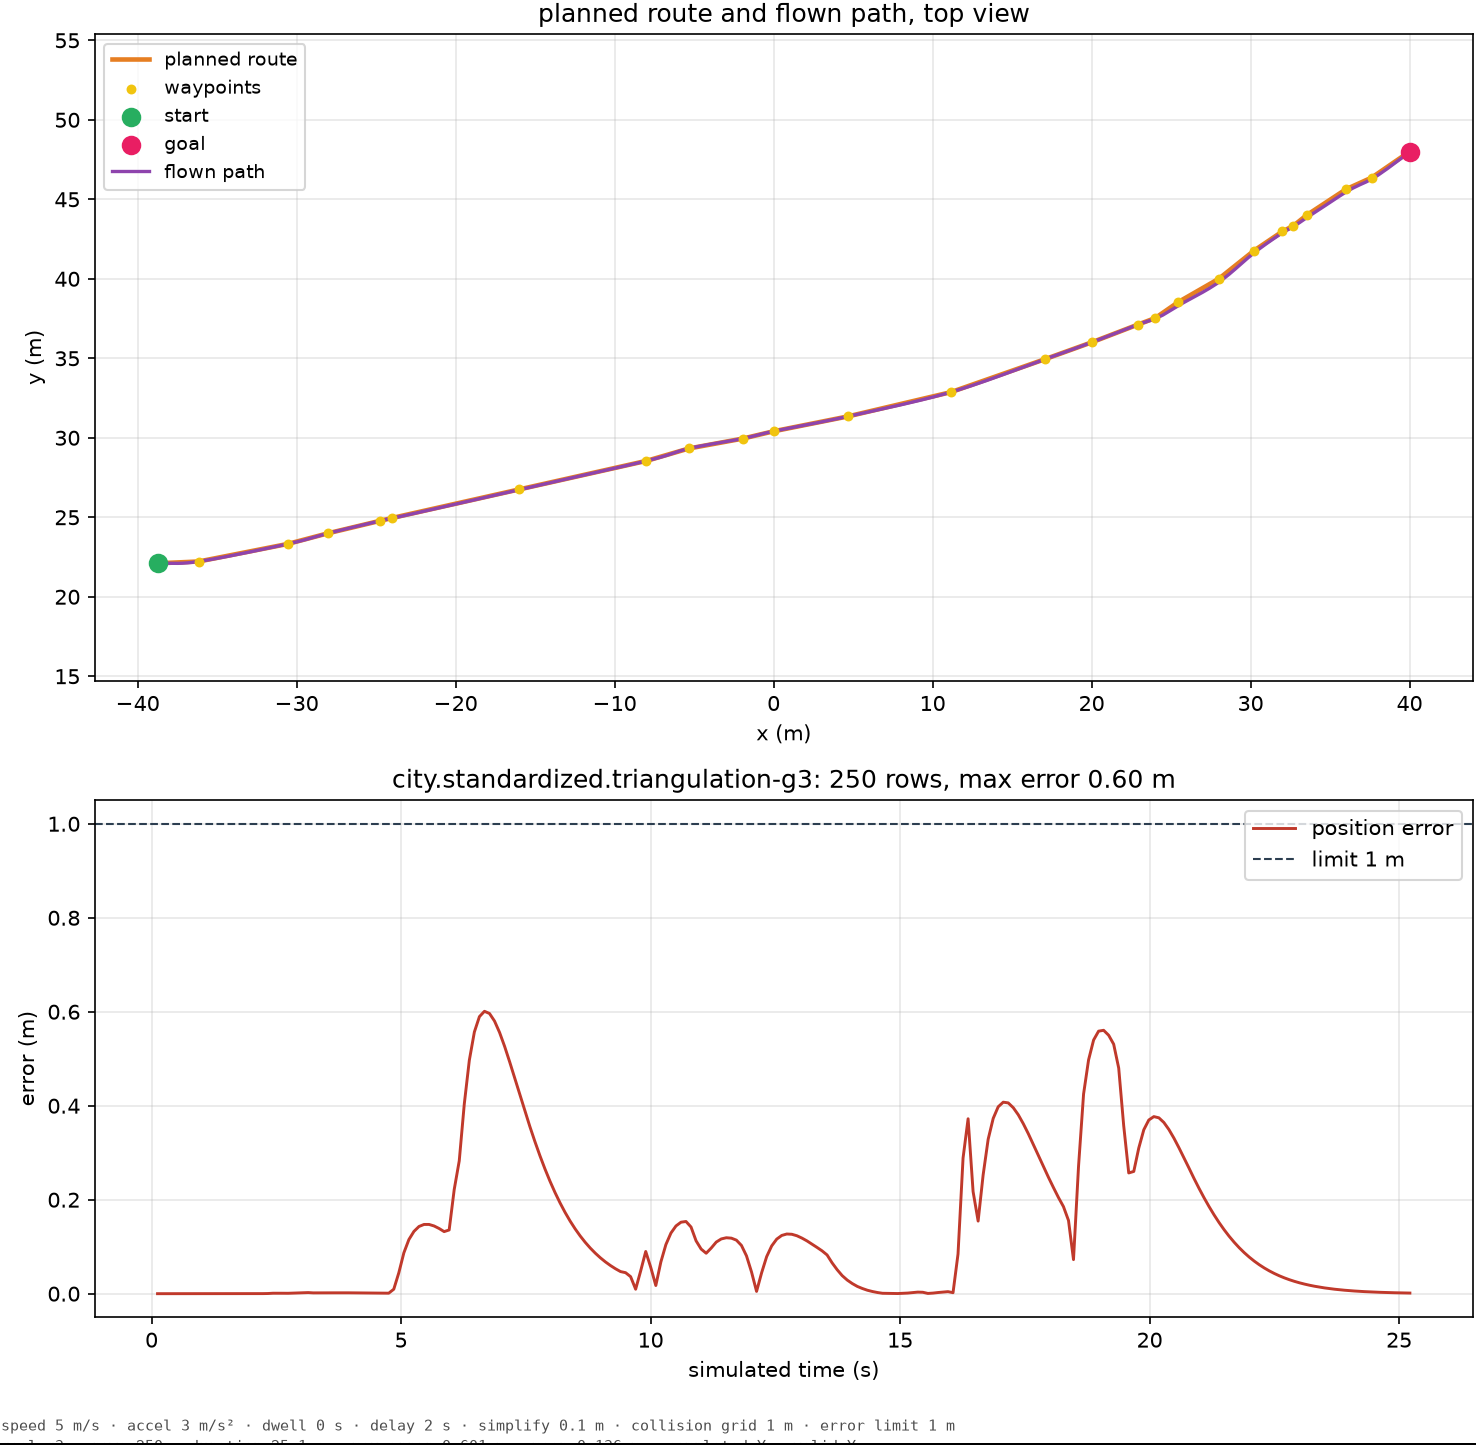
\includegraphics[width=\linewidth]{Figures/crop/cell4_g3_tracking.png}
    \caption{Lưới $4$, G3: $e_{\max}=0{,}601$, đạt mốc.}
  \end{subfigure}
  \caption{Đường đã bay và sai số của hai đích còn lại trên lưới $4$: G1 (trên)
    và G3 (dưới). Cả hai đều nằm dưới mốc $1$ đơn vị.}
  \label{fig:tracking-g1g3}
\end{figure*}

Hình~\ref{fig:tracking-g1g3} cho thấy G1 và G3 có cùng dạng sai số: gần như
phẳng trên đoạn thẳng, tăng ở các góc cua rồi giảm khi ra khỏi góc. G3 có nhiều
đỉnh hơn vì tuyến có nhiều waypoint và một đoạn ngắn $0{,}777$; đỉnh lớn nhất
$0{,}601$ vẫn dưới mốc. G1 có ít đỉnh hơn và sai số lớn nhất $0{,}399$, phù hợp
với khoảng cách waypoint đều hơn.

\begin{figure*}[!t]
  \centering
  \begin{subfigure}{0.45\textwidth}
    \centering
    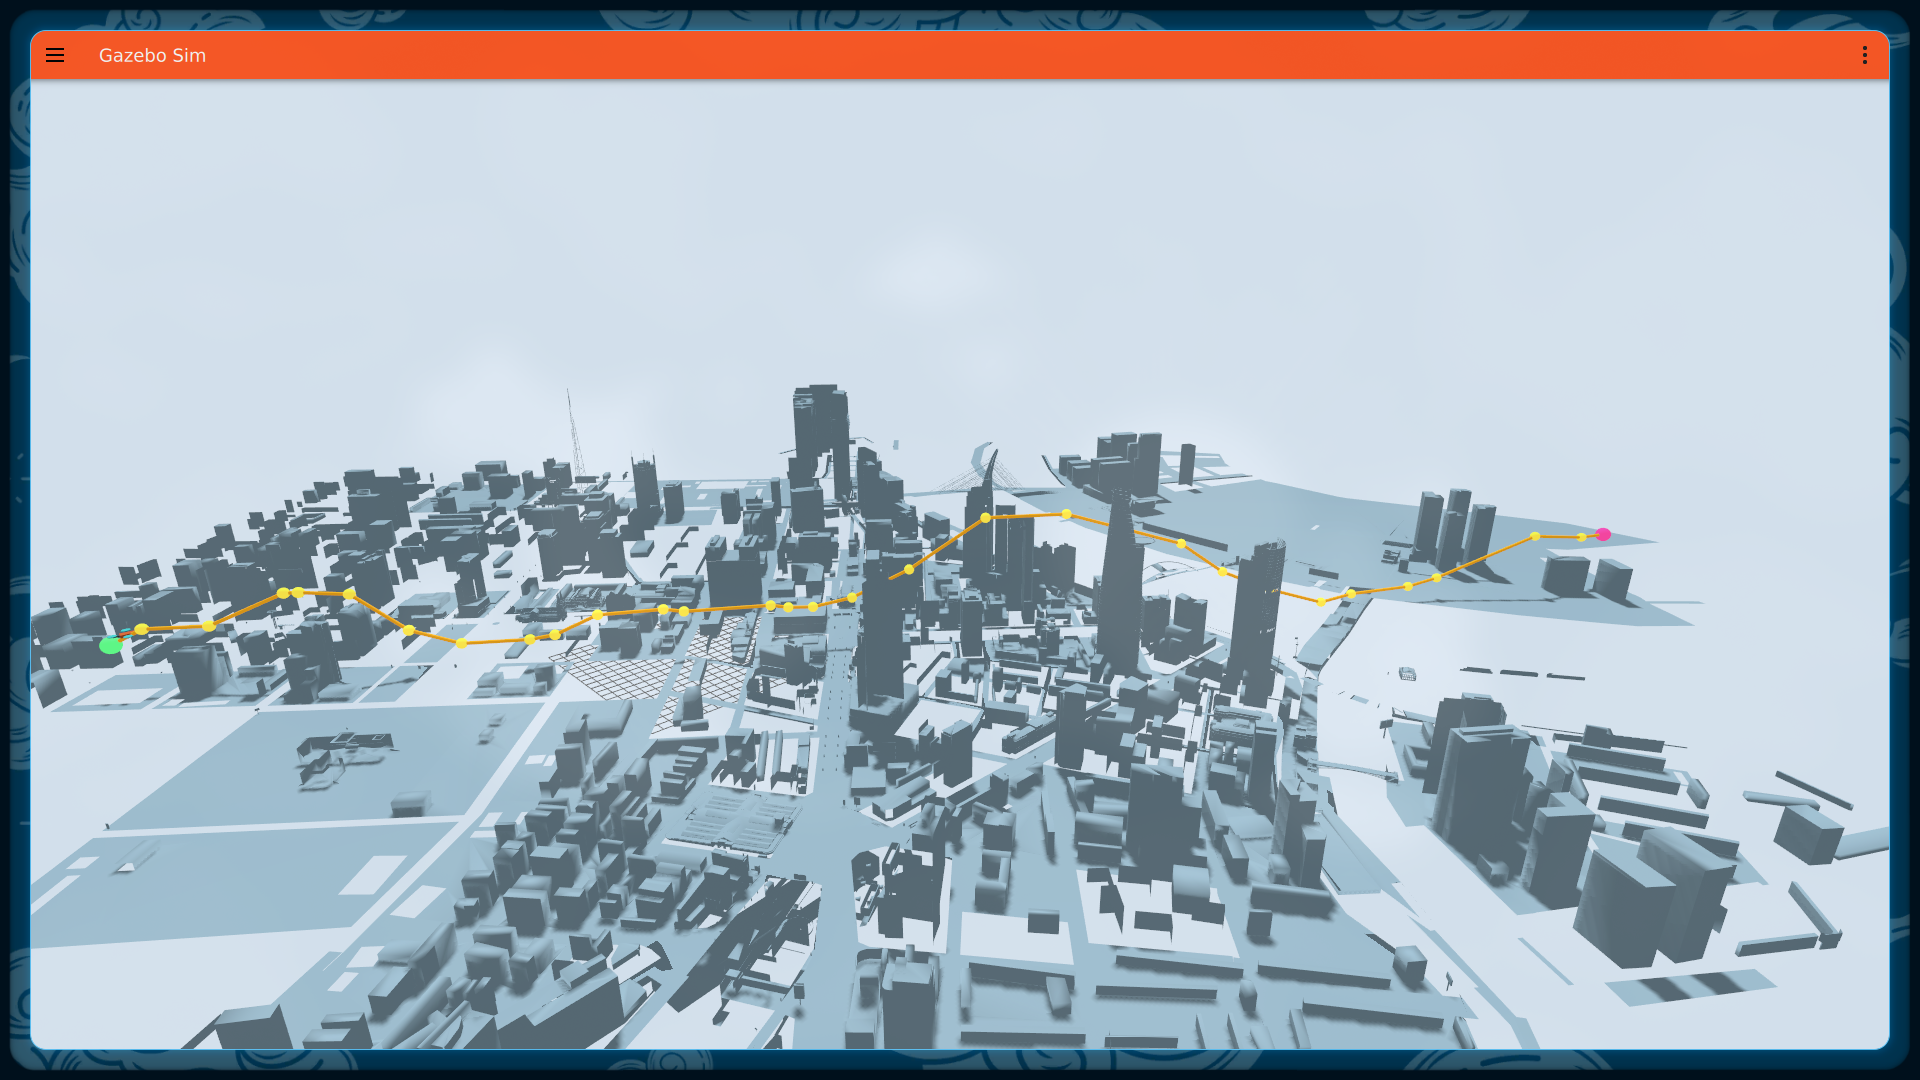
\includegraphics[width=\linewidth]{Figures/crop/gazebo_g1_city.png}
    \caption{G1, toàn cảnh.}
  \end{subfigure}\hfill
  \begin{subfigure}{0.45\textwidth}
    \centering
    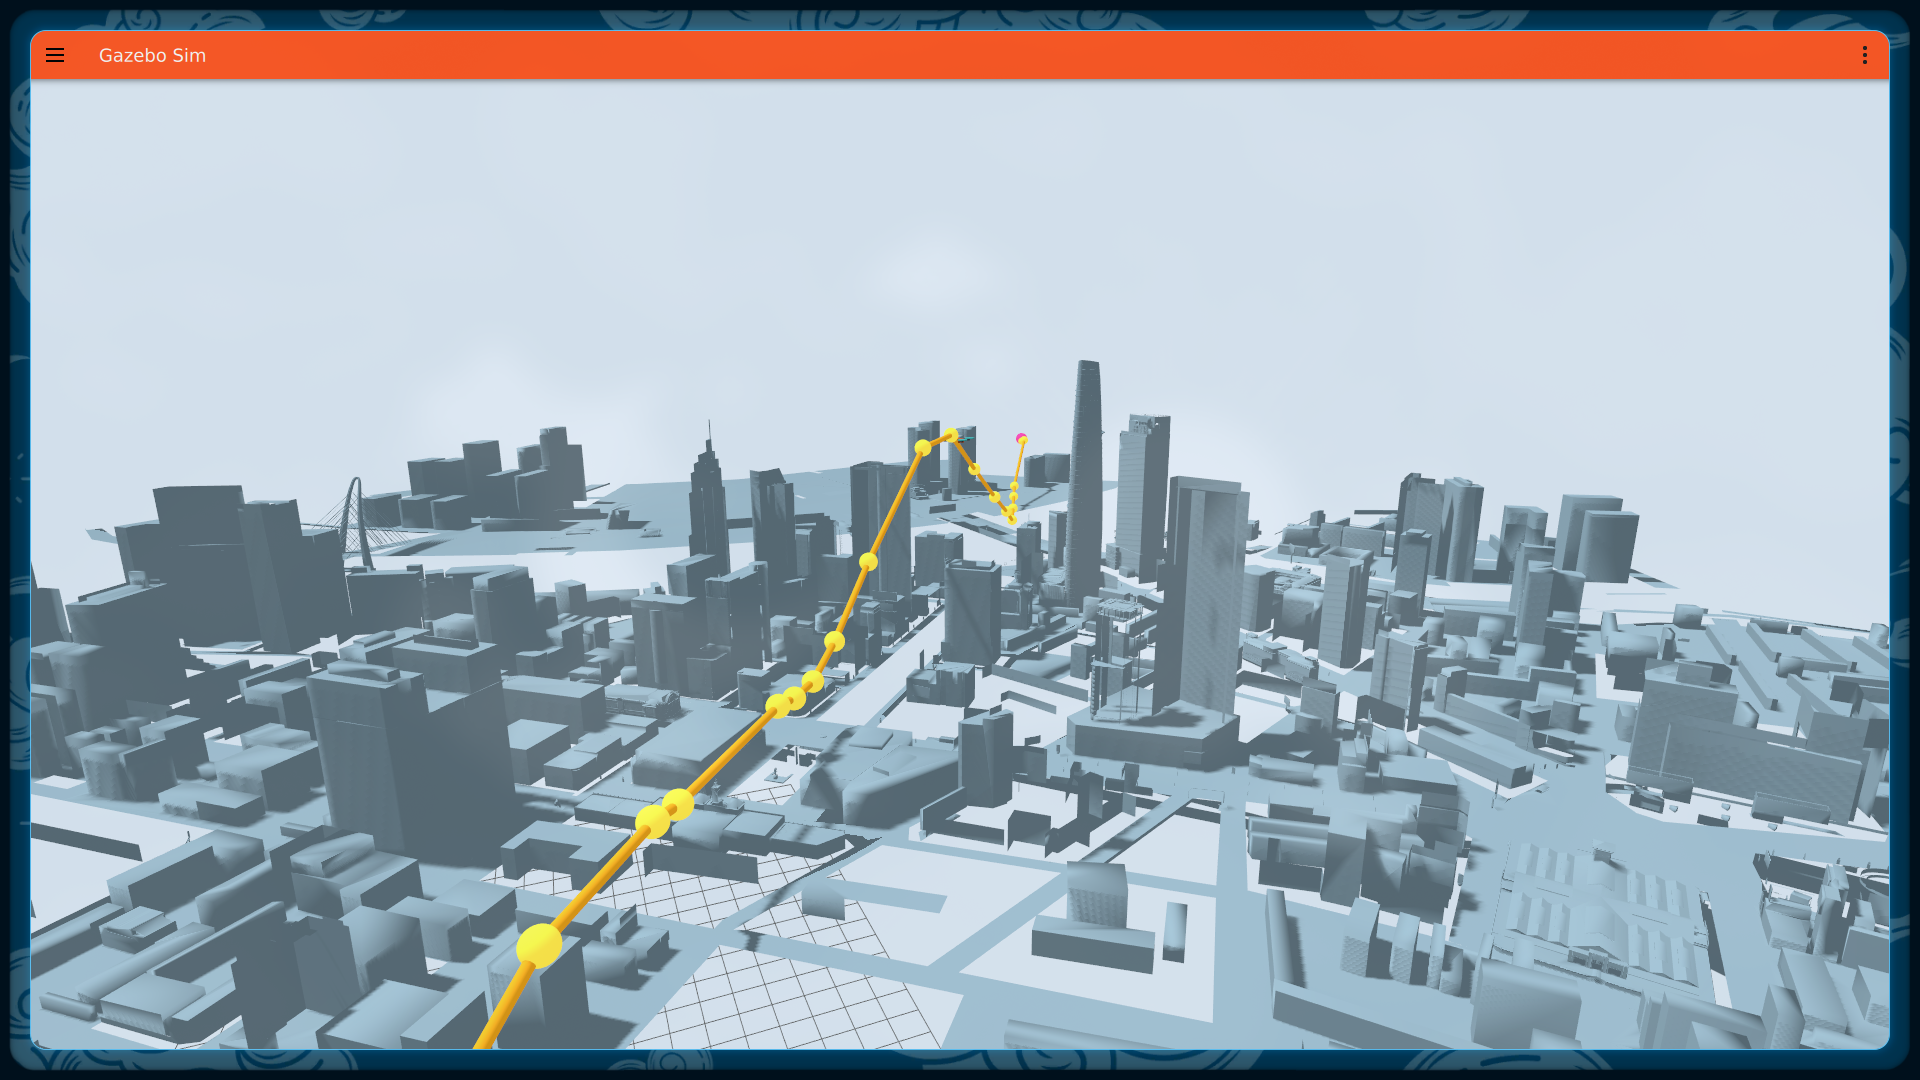
\includegraphics[width=\linewidth]{Figures/crop/gazebo_g1_close.png}
    \caption{G1, cận cảnh.}
  \end{subfigure}\par\vspace{2pt}
  \begin{subfigure}{0.45\textwidth}
    \centering
    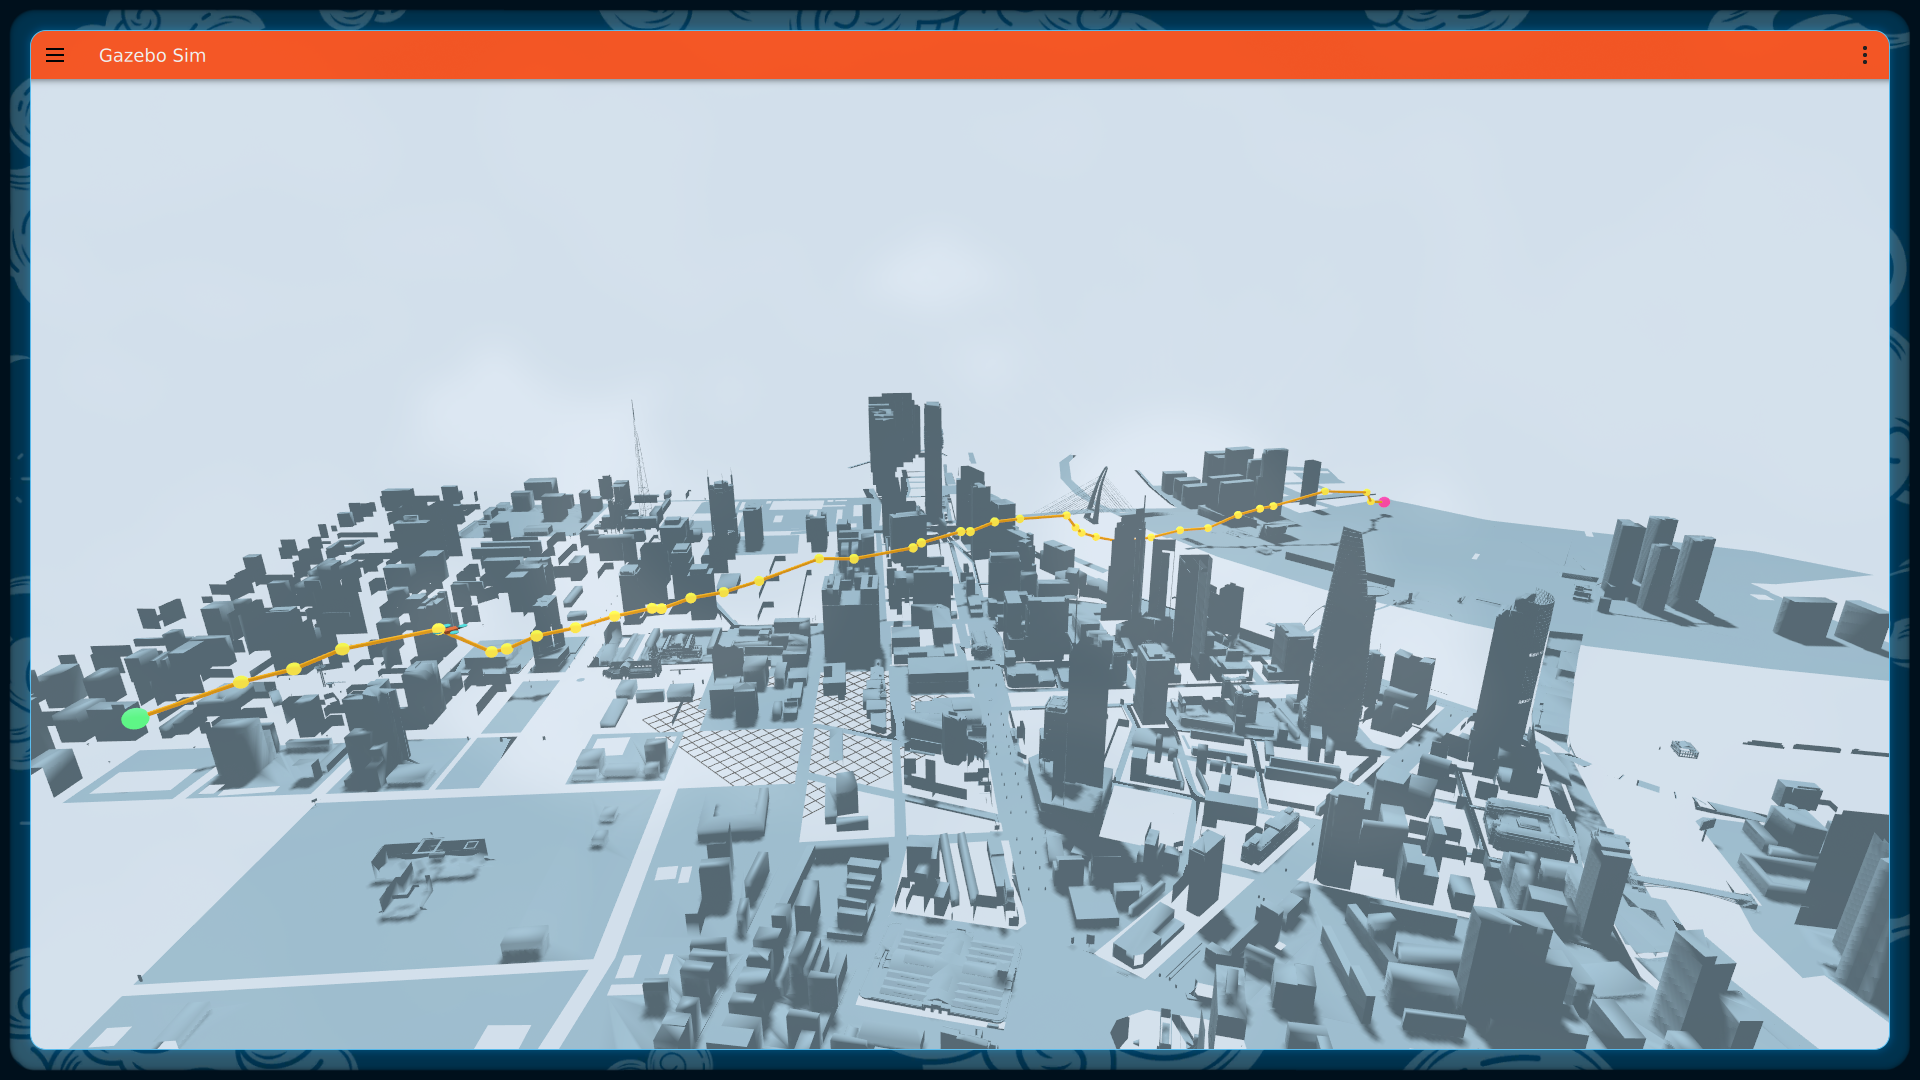
\includegraphics[width=\linewidth]{Figures/crop/gazebo_g2_city.png}
    \caption{G2, toàn cảnh.}
  \end{subfigure}\hfill
  \begin{subfigure}{0.45\textwidth}
    \centering
    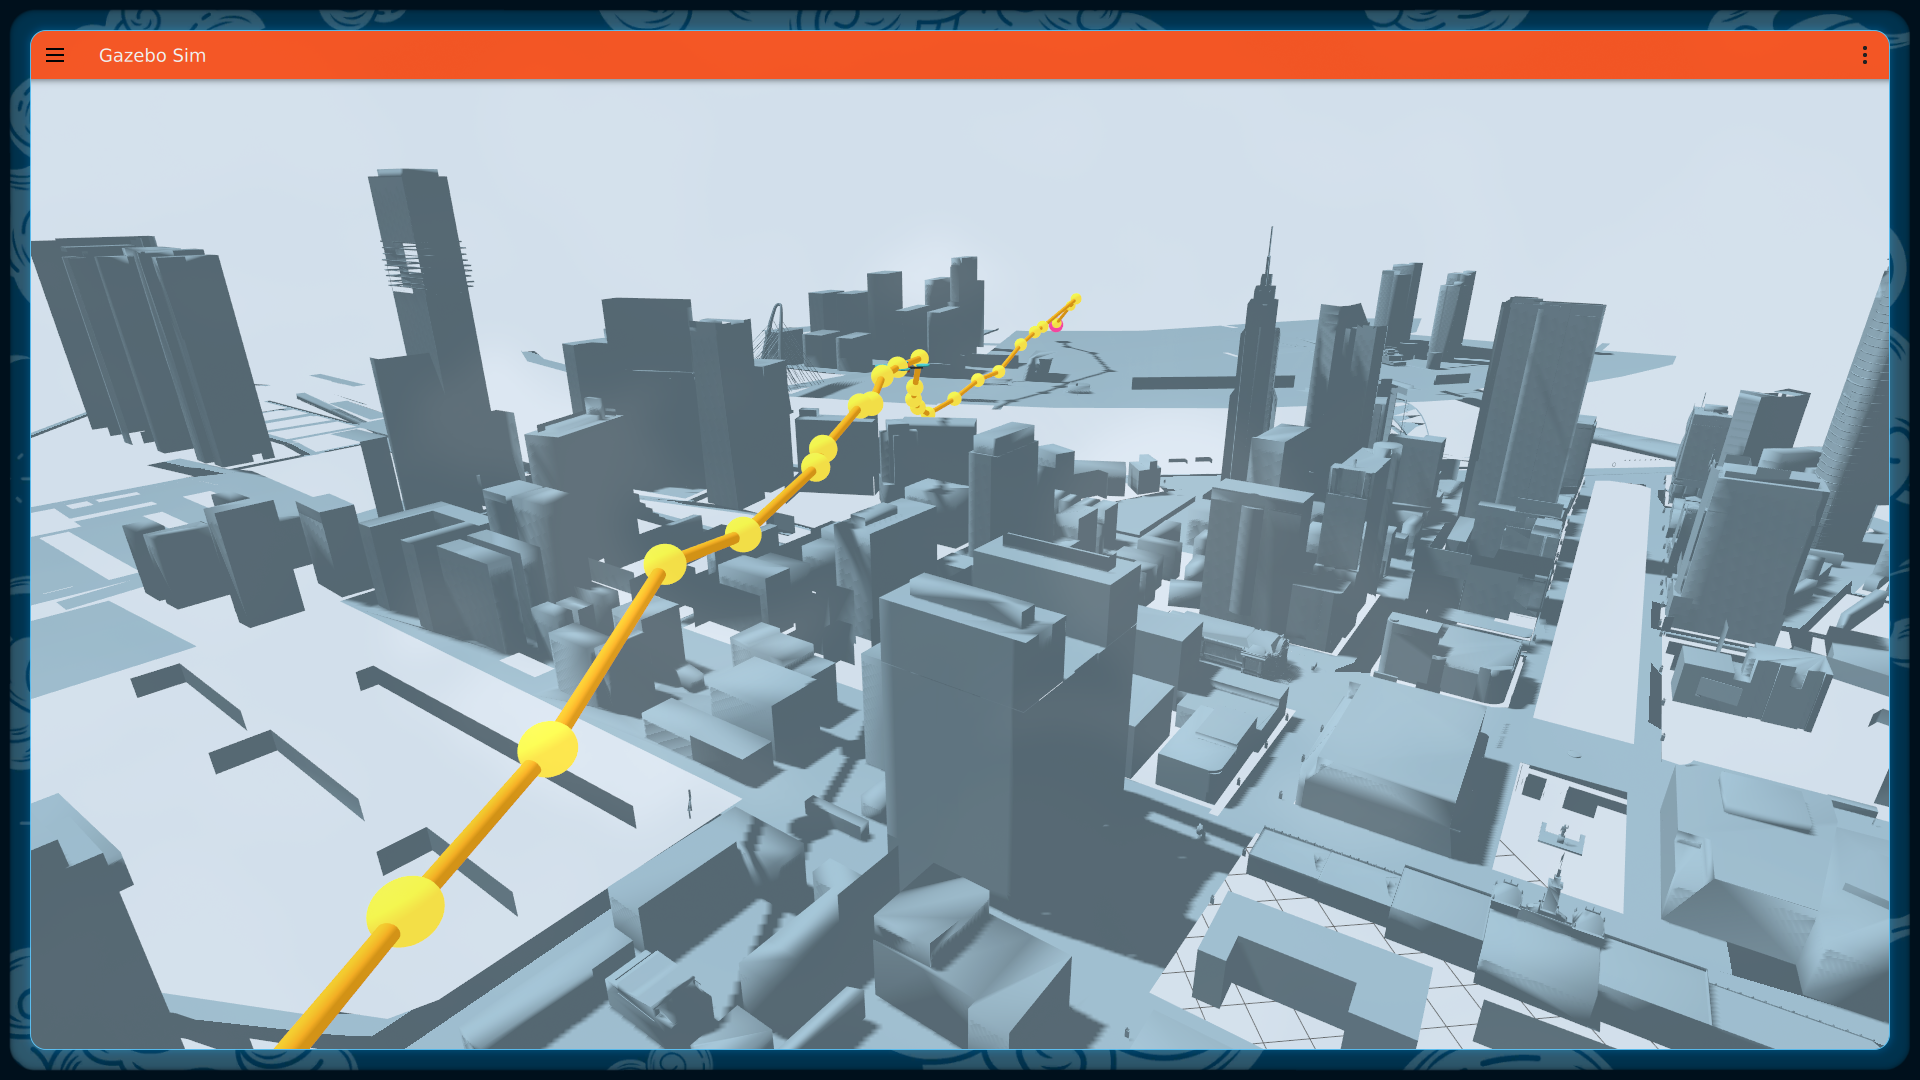
\includegraphics[width=\linewidth]{Figures/crop/gazebo_g2_close.png}
    \caption{G2, cận cảnh.}
  \end{subfigure}\par\vspace{2pt}
  \begin{subfigure}{0.45\textwidth}
    \centering
    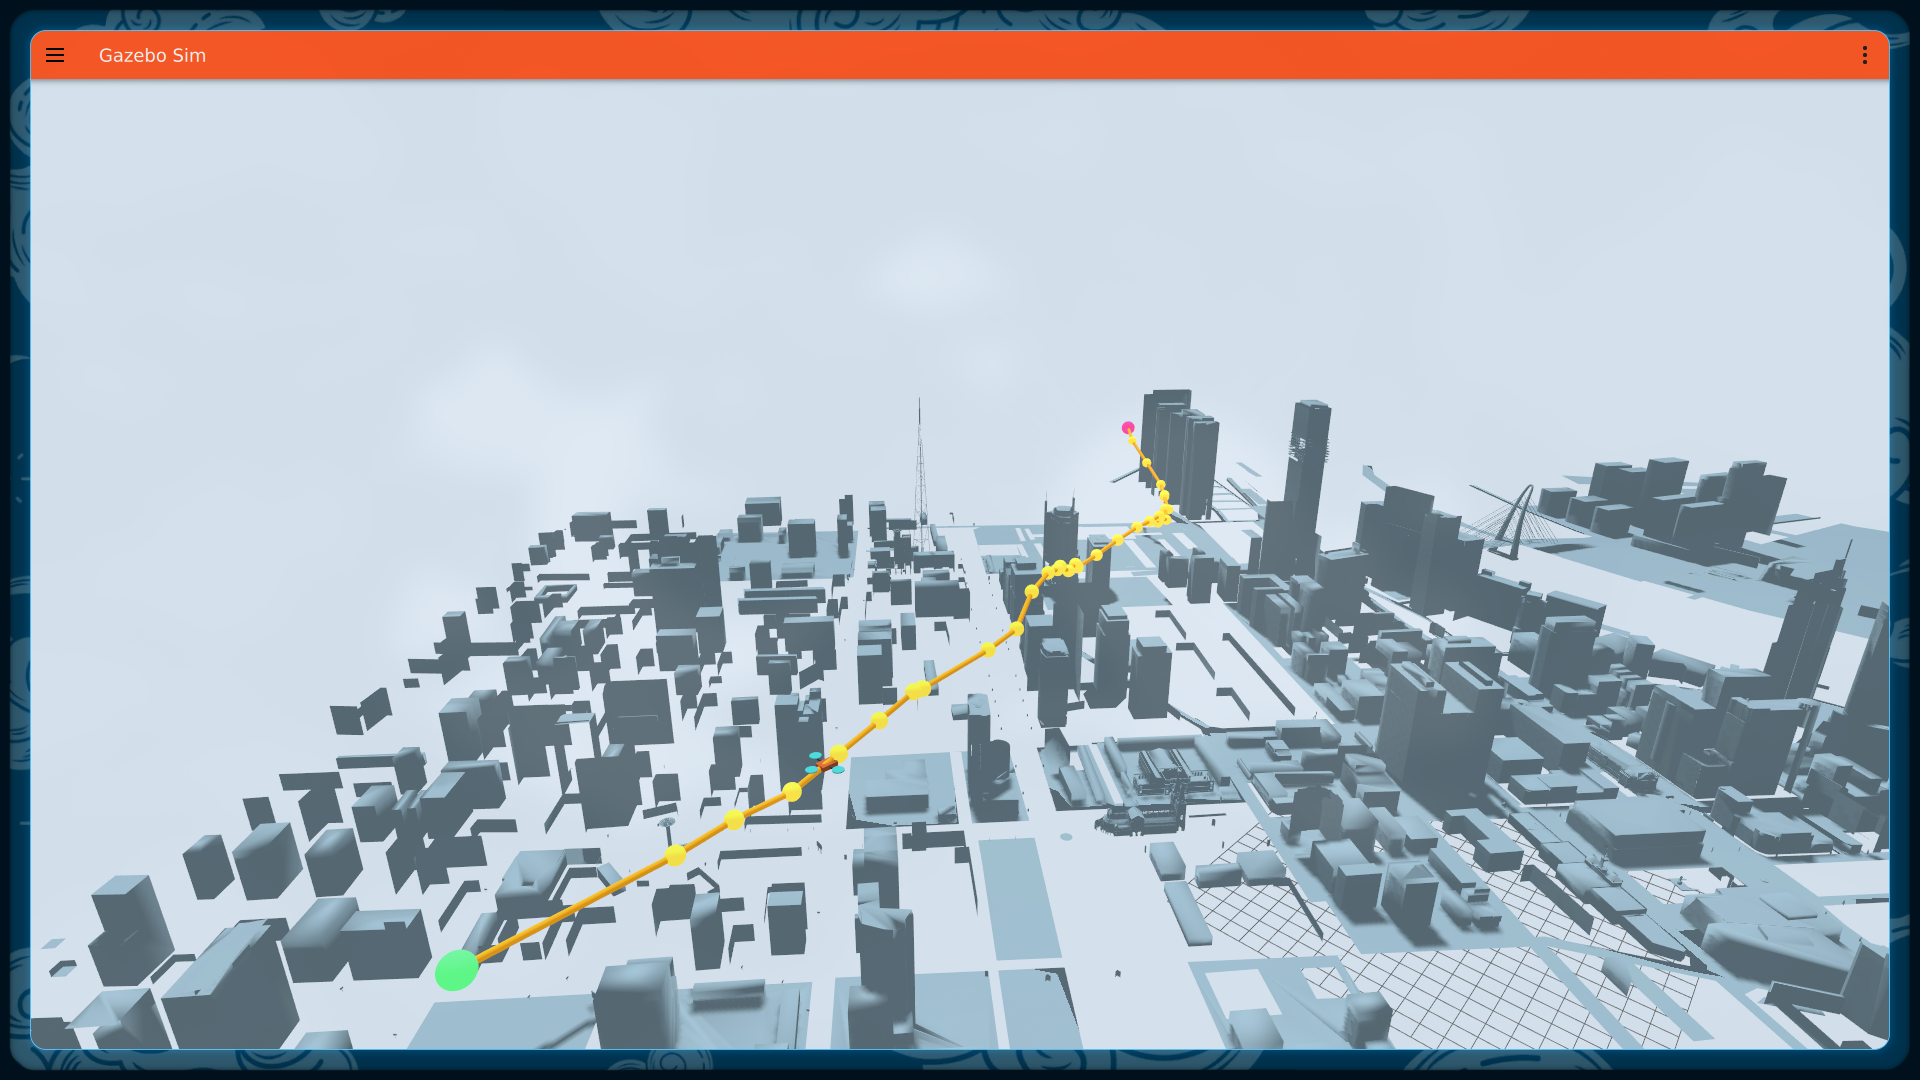
\includegraphics[width=\linewidth]{Figures/crop/gazebo_g3_city.png}
    \caption{G3, toàn cảnh.}
  \end{subfigure}\hfill
  \begin{subfigure}{0.45\textwidth}
    \centering
    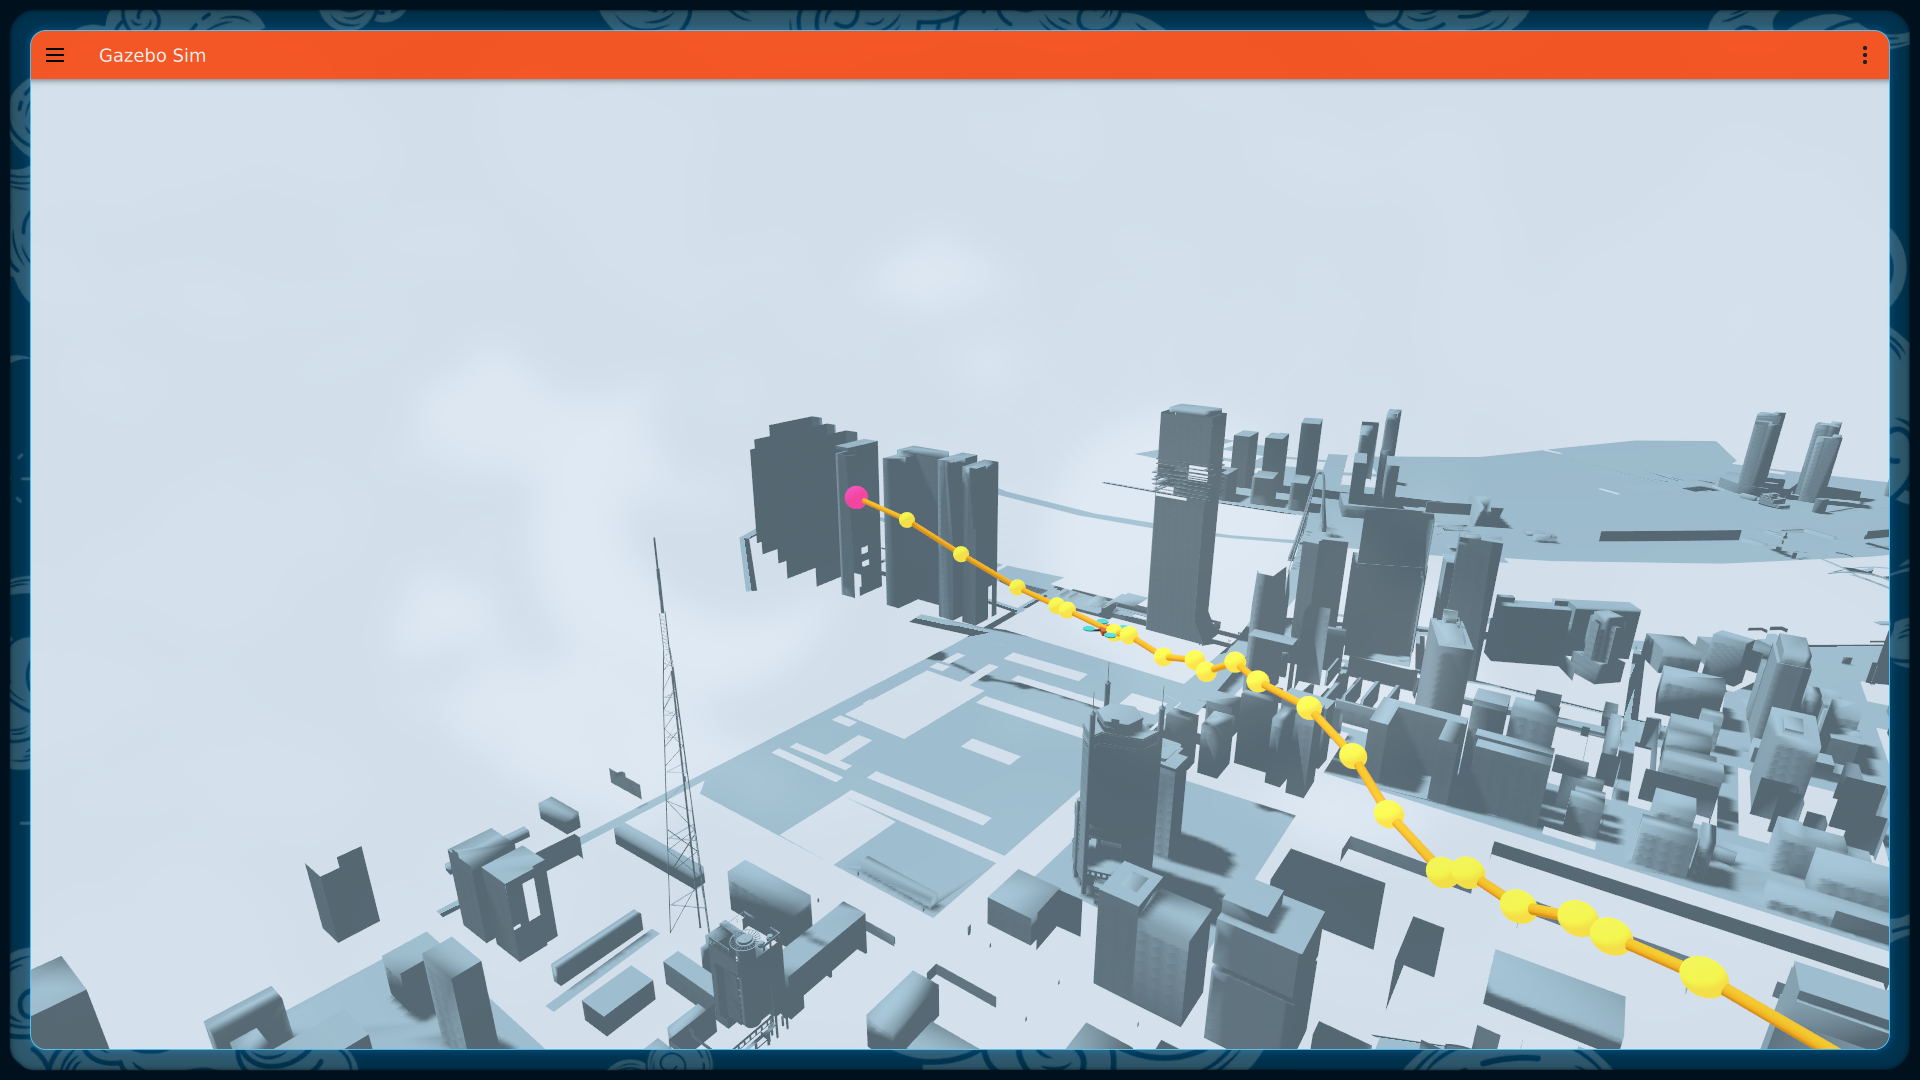
\includegraphics[width=\linewidth]{Figures/crop/gazebo_g3_close.png}
    \caption{G3, cận cảnh.}
  \end{subfigure}
  \caption{Giao diện Gazebo trong ba phiên G1, G2 và G3: thành phố, tuyến kế
    hoạch màu cam, waypoint vàng, điểm xuất phát xanh và đích hồng. Ảnh chụp
    giao diện chỉ để minh họa; kết luận định lượng lấy từ telemetry.}
  \label{fig:gazebo-g1}
\end{figure*}

Hình~\ref{fig:gazebo-g1} cho thấy cả ba tuyến đều đi qua các khe phố và bám theo
cao độ công trình; các waypoint vàng nằm trên mái hoặc sát mặt envelope, không đi
xuyên qua khối nhà. G1 đi gần như thẳng theo hướng đông-nam; G2 có một đoạn leo
lên tháp cao rồi xuống; G3 đi về phía đông-bắc và có nhiều đoạn đổi hướng hơn.
Các ảnh này chỉ minh họa giao diện, không dùng để đo sai số.

\begin{table*}[!t]
  \caption{Thống kê khoảng cách waypoint trên tuyến đã rút gọn mà plugin thực sự
    bay. $n$ là số waypoint; $d_{\min}$, $d_{\rm med}$, $d_{\max}$ là khoảng cách
    đoạn ngắn nhất, trung vị và dài nhất; $r_{\max}$ là tỉ lệ lớn nhất giữa độ dài
    tiếp tuyến Catmull--Rom và đoạn ngắn kề nó.}
  \label{tab:waypoints}
  {\fontsize{7}{8.6}\selectfont
  \begin{adjustbox}{max width=\textwidth}
  \begin{tabular}{@{}llrrrrr@{}}
    \toprule
    Cấu hình & Goal & $n$ & $d_{\min}$ & $d_{\rm med}$ & $d_{\max}$ & $r_{\max}$ \\
    \midrule
    lưới $5$ & g1 & 27 & 1,389 & 5,633 & 12,766 & 3,36 \\
             & g2 & 25 & 1,264 & 3,705 & 19,464 & 7,60 \\
             & g3 & 24 & 1,217 & 3,533 & 10,347 & 1,65 \\
    \midrule
    lưới $4$ & g1 & 27 & 1,595 & 4,804 & 15,624 & 2,92 \\
             & g2 & 24 & 1,545 & 4,431 & 13,600 & 3,15 \\
             & g3 & 26 & 0,777 & 2,935 &  8,208 & 5,40 \\
    \midrule
    lưới $3$ & g1 & 30 & 1,119 & 4,925 & 11,887 & 3,24 \\
             & g2 & 38 & 0,801 & 3,102 &  8,988 & 3,62 \\
             & g3 & 33 & 0,776 & 2,783 &  8,760 & 4,40 \\
    \bottomrule
  \end{tabular}
  \end{adjustbox}}
\end{table*}

\begin{table*}[!t]
  \caption{Phân rã sai số tại một số thời điểm của G2 trên lưới $3$. $z$ và
    $z_{\rm ref}$ là cao độ đo và cao độ tham chiếu; $\Delta z$ là thành phần
    đứng; tỉ lệ đứng là $|\Delta z|/e$.}
  \label{tab:g2vertical}
  {\fontsize{7}{8.6}\selectfont
  \begin{tabular}{@{}rrrrrrrr@{}}
    \toprule
    $t$ (s) & $z$ & $z_{\rm ref}$ & $\Delta z$ & $e$ & Tỉ lệ đứng
      & $v_z$ & $v_{z,\rm ref}$ \\
    \midrule
    7,285 & 7,032 & 6,765 & $+0{,}268$ & 0,269 & 99,6\,\% & $-3{,}498$ & $-3{,}569$ \\
    7,891 & 5,668 & 6,648 & $-0{,}980$ & 0,987 & 99,3\,\% & $-0{,}530$ & $+2{,}083$ \\
    8,092 & 5,678 & 7,017 & $-1{,}339$ & 1,348 & 99,4\,\% & $+0{,}524$ & $+1{,}383$ \\
    8,193 & 5,741 & 7,115 & $-1{,}374$ & 1,381 & 99,5\,\% & $+0{,}682$ & $+0{,}537$ \\
    8,294 & 5,806 & 7,129 & $-1{,}323$ & 1,326 & 99,7\,\% & $+0{,}560$ & $-0{,}164$ \\
    \bottomrule
  \end{tabular}}
\end{table*}

Không có cấu hình nào nhỏ nhất ở mọi đích: lưới $5$ có sai số G1 thấp nhất
($0{,}365$), lưới $3$ có sai số G3 thấp nhất ($0{,}580$), còn lưới $4$ chỉ nhỉnh
hơn ở hai đích này nhưng là cấu hình duy nhất đạt mốc ở cả ba. Vì vậy nên đọc kết
quả theo tiêu chí đã đặt trước (đạt $1$ đơn vị ở mọi đích) thay vì chọn cấu hình
theo một con số sai số đơn lẻ.

\subsection{So sánh ba cấu hình và tái lập}\label{sec:archive}

Ba cấu hình được lưu thành ba bộ kết quả độc lập, không ghi đè lên nhau. Mỗi bộ
gồm bề mặt, route, world, telemetry, ảnh và một bản kê khai tham số cùng SHA của
mọi tệp. Nhờ vậy có thể so sánh sau khi lần chạy mới nhất đã thay đổi thư mục làm
việc. Bảng~\ref{tab:summary} tóm tắt ba cấu hình; Hình~\ref{fig:routes} so sánh
tuyến trên lưới $4$ và lưới $3$.

\begin{table*}[!t]
  \caption{Tóm tắt ba cấu hình: kích thước lưới, thời gian lập tuyến, số lần lan
    truyền, sai số lớn nhất từng đích và số đích đạt mốc $1$.}
  \label{tab:summary}
  {\fontsize{7}{8.6}\selectfont
  \begin{adjustbox}{max width=\textwidth}
  \begin{tabular}{@{}lrrrrrrl@{}}
    \toprule
    Cấu hình & $V/F$ & $T_{\rm plan}$ (s) & $\sum P$
      & $e_{\max}$ G1 & $e_{\max}$ G2 & $e_{\max}$ G3 & Đạt mốc \\
    \midrule
    lưới $5$ & 2\,295/4\,400 & 44,984 & 104 & 0,365 & 1,022 & 0,852 & 2/3 \\
    lưới $4$ & 3\,355/6\,480 & 186,175 & 187 & 0,399 & 0,591 & 0,601 & 3/3 \\
    lưới $3$ & 5\,913/11\,520 & 1\,008,389 & 429 & 0,508 & 1,381 & 0,580 & 2/3 \\
    \bottomrule
  \end{tabular}
  \end{adjustbox}}
\end{table*}

\begin{figure*}[!t]
  \centering
  \begin{subfigure}{0.70\textwidth}
    \centering
    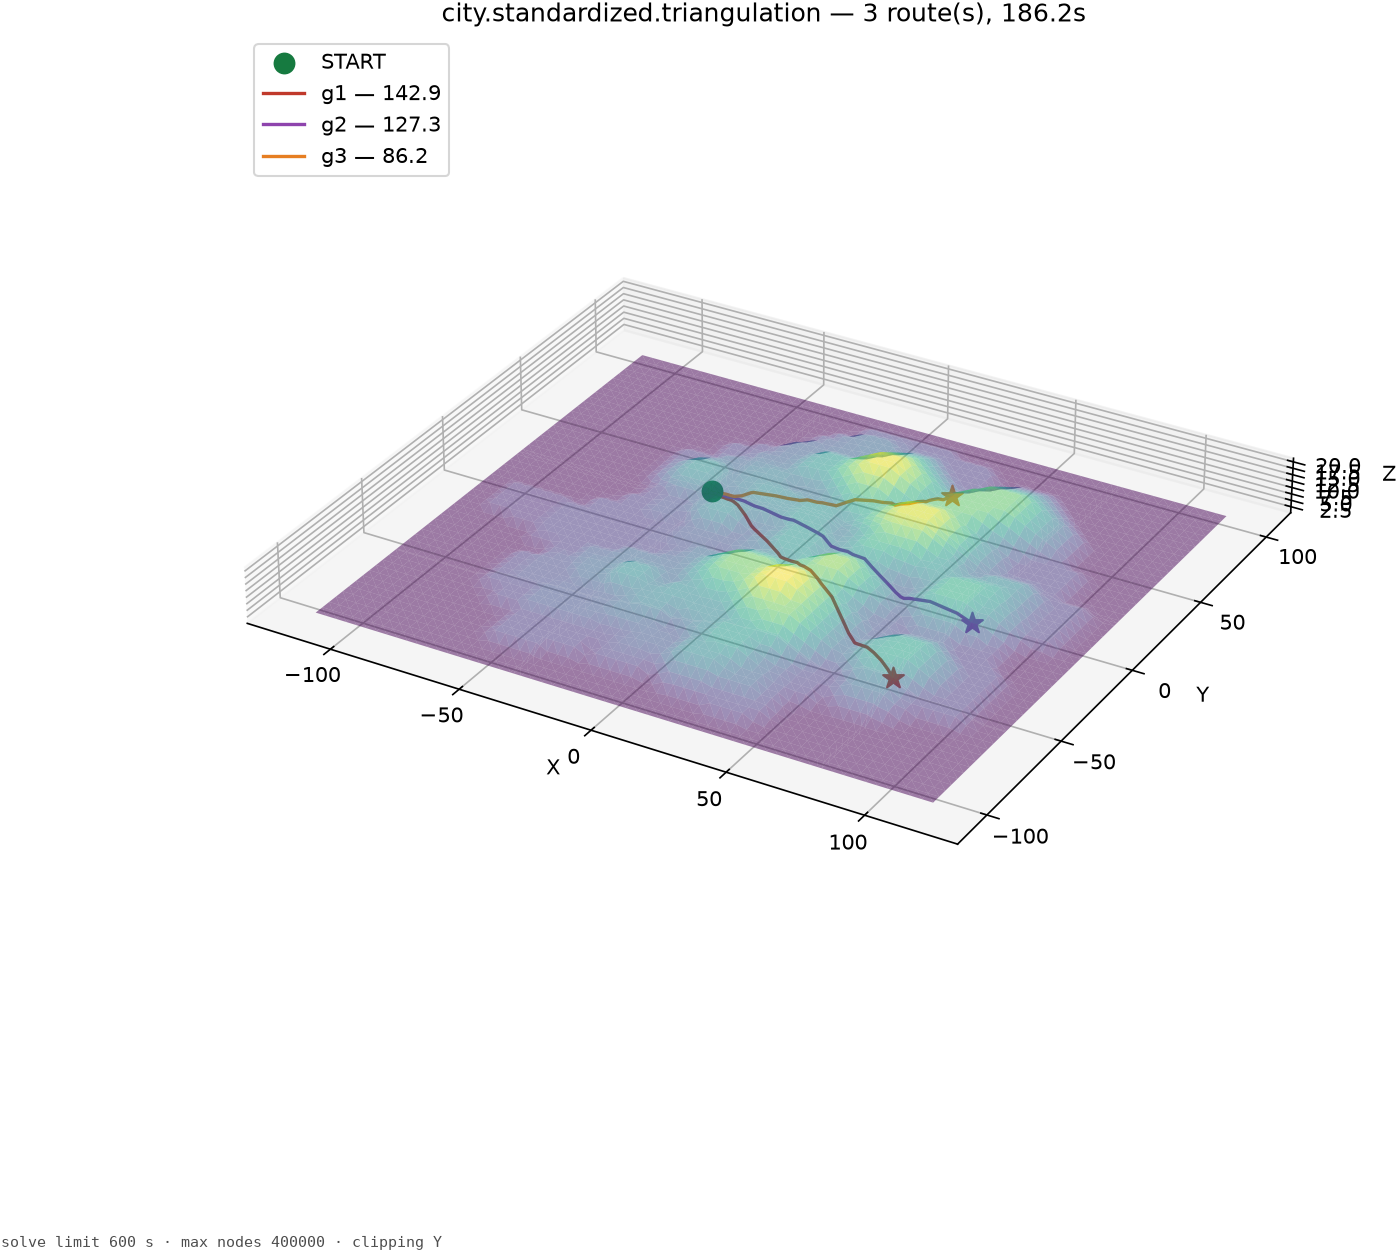
\includegraphics[width=\linewidth]{Figures/crop/cell4_routes.png}
    \caption{Lưới $4$: G1 $142{,}909050$, G2 $127{,}295935$, G3 $86{,}194146$.}
  \end{subfigure}\par\vspace{2pt}
  \begin{subfigure}{0.70\textwidth}
    \centering
    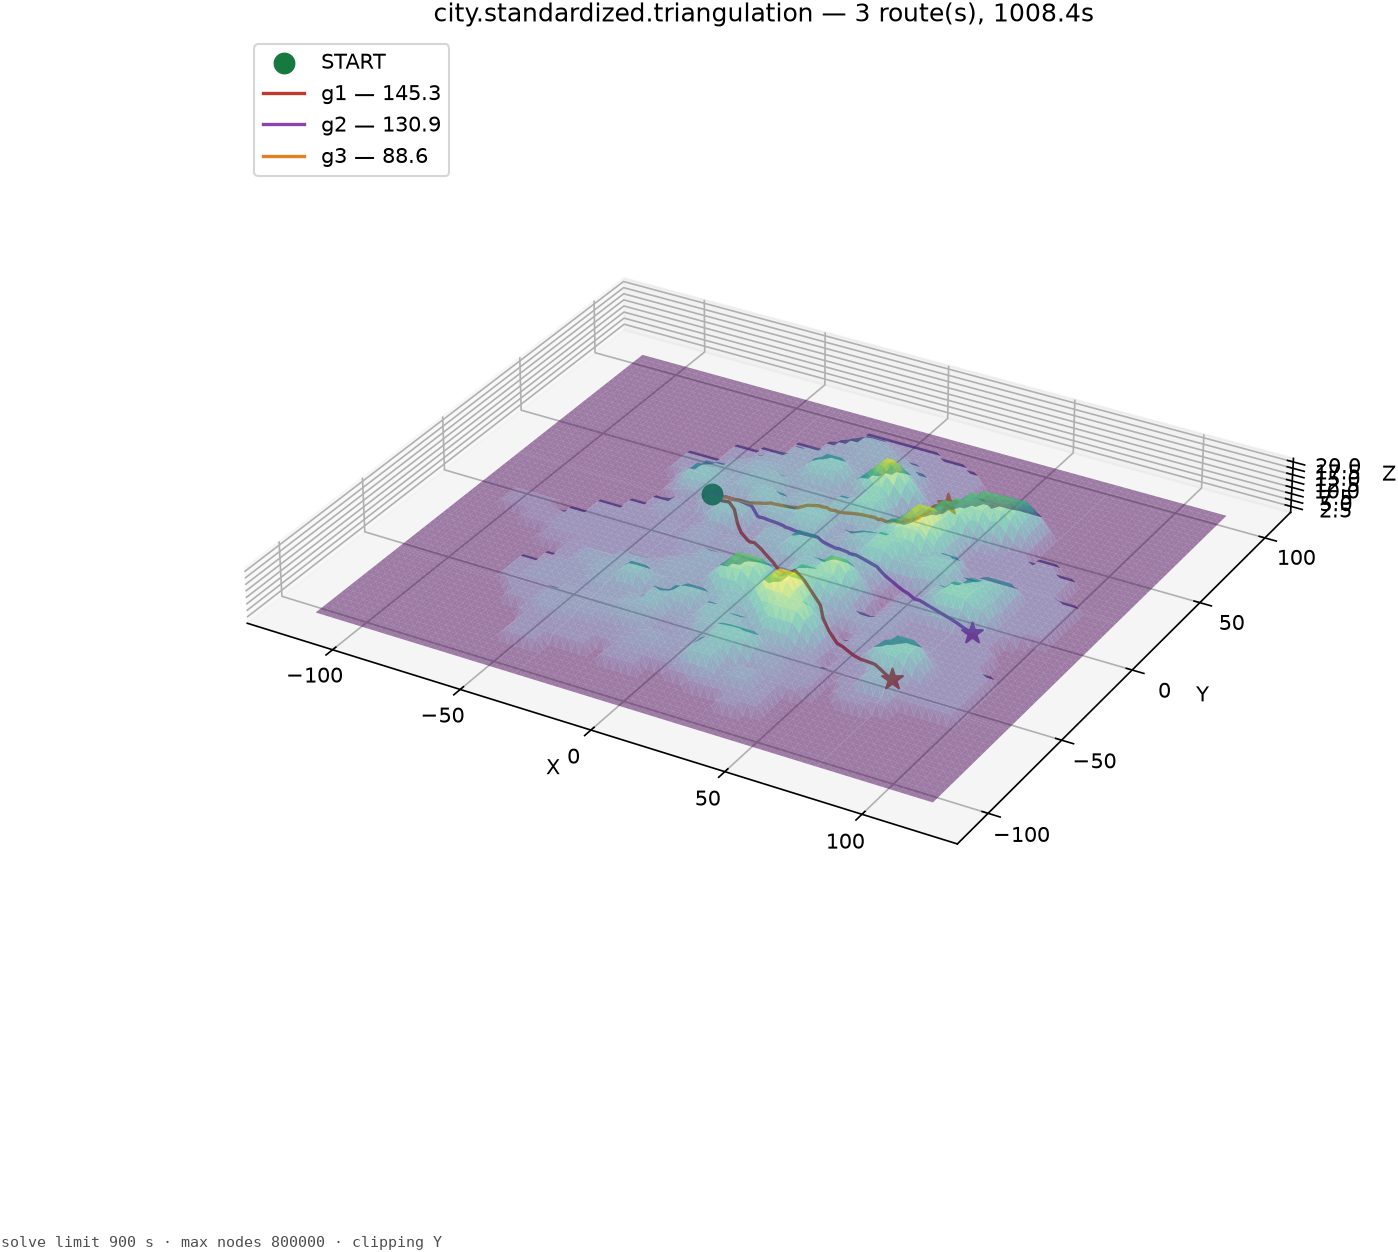
\includegraphics[width=\linewidth]{Figures/crop/cell3_routes.png}
    \caption{Lưới $3$: G1 $145{,}314559$, G2 $130{,}891670$, G3 $88{,}611502$.}
  \end{subfigure}
  \caption{Ba tuyến trên hai bề mặt. Lưới $4$ (trên) là cấu hình duy nhất đạt mốc
    bám tuyến $1$ ở cả ba đích; lưới $3$ (dưới) có bề mặt sát hình học hơn và
    tuyến dài hơn.}
  \label{fig:routes}
\end{figure*}

Hình~\ref{fig:routes} so sánh trực tiếp hai bề mặt. Ba tuyến trên lưới $3$ dài
hơn tuyến tương ứng trên lưới $4$ khoảng $2{,}4$; $3{,}6$ và $2{,}4$ đơn vị, trong
khi hình dạng tổng thể vẫn tương tự: cùng xuất phát từ một nguồn, cùng ba hướng
đích, nhưng lưới $3$ bám sát khối công trình hơn nên có thêm các đoạn lượn và
điểm đích bị snap xa hơn. Đây là lý do không thể quy toàn bộ chênh lệch độ dài
cho kích thước ô.

Hình~\ref{fig:routes-detail} cho thấy tuyến không đi theo mặt phẳng: khi bề mặt
có một tháp cao, tuyến leo lên theo ramp rồi xuống phía bên kia; các đoạn gãy
tương ứng với cạnh tam giác. Hình chiếu bằng xác nhận ba tuyến tách nhau ngay sau
nguồn và chỉ gặp lại ở vùng gần đích, phù hợp với việc mỗi goal được tìm trong
một lượt riêng.

\begin{figure*}[!t]
  \centering
  \begin{subfigure}{0.48\textwidth}
    \centering
    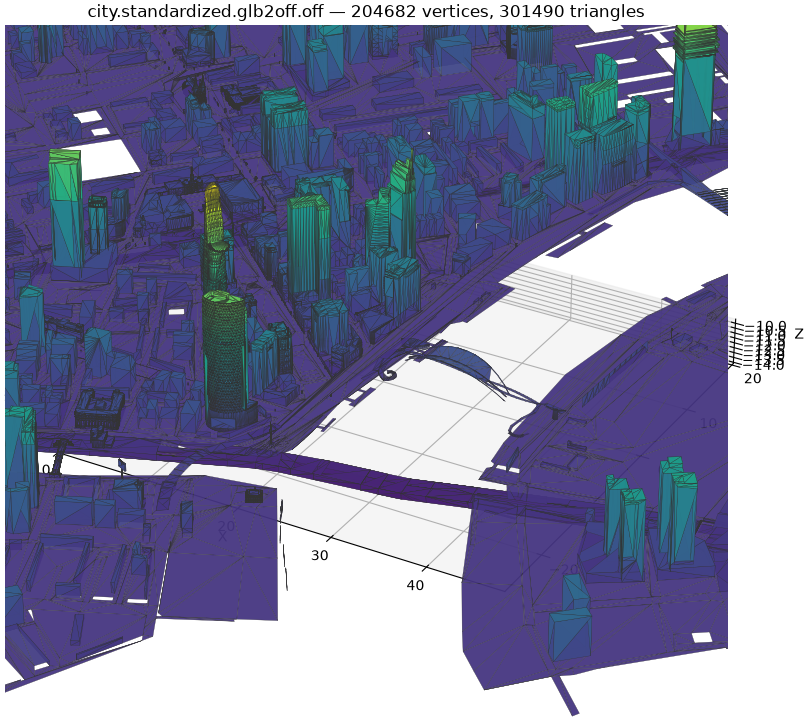
\includegraphics[width=\linewidth]{Figures/crop/etc_city_wide.png}
    \caption{Toàn cảnh vùng trung tâm.}
  \end{subfigure}\hfill
  \begin{subfigure}{0.48\textwidth}
    \centering
    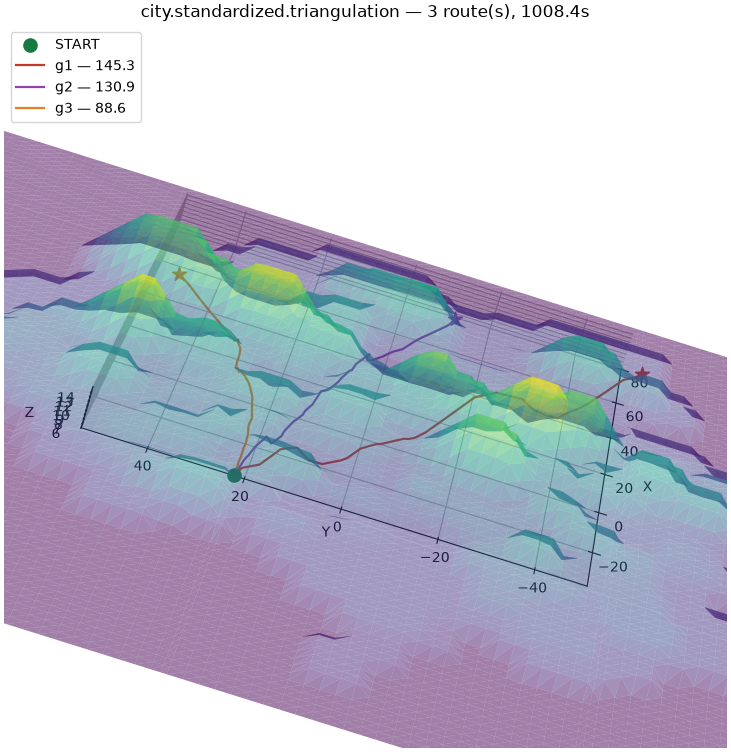
\includegraphics[width=\linewidth]{Figures/crop/etc_routes_3d_alt.png}
    \caption{Góc nhìn 3D khác của ba tuyến.}
  \end{subfigure}
  \caption{Hai góc nhìn bổ sung: toàn cảnh vùng trung tâm và một góc 3D khác của
    ba tuyến trên bề mặt lưới $3$ m.}
  \label{fig:extra-views}
\end{figure*}

Hình~\ref{fig:extra-views} cho thấy cùng một dữ liệu nhưng ở hai tỉ lệ: toàn cảnh
giúp thấy tuyến đi qua các khu phố khác nhau, còn góc 3D thứ hai làm rõ các đoạn
leo dốc và đổi hướng. Cả hai đều củng cố nhận xét rằng tuyến không đi theo mặt
phẳng và phải bám theo envelope.

\subsection{Những kết luận rút ra từ toàn bộ quy trình}\label{sec:lessons}

Sau khi chạy trọn quy trình từ scene thô đến telemetry, có thể rút ra sáu kết
luận vận hành, bên cạnh các số liệu ở trên.

\begin{enumerate}
  \item \textbf{Quy trình ba giai đoạn là một chuỗi kiểm chứng, không chỉ là ba
    lệnh.} Mỗi giai đoạn ghi hash của đầu vào và đầu ra; bộ kết quả lưu cả bản kê
    khai. Nhờ đó một con số trong bài truy ngược được về đúng scene, bề mặt,
    mission, route và telemetry. Đây là điều kiện cần để kết quả mô phỏng được
    xem là bằng chứng, không chỉ là ảnh minh họa.
  \item \textbf{Chọn kích thước ô là bài toán cân bằng, không phải ``càng mịn càng
    tốt''.} Lưới $5$ m đủ nhanh nhưng waypoint không đều ở G2; lưới $4$ m là cấu
    hình duy nhất đạt mốc $1$ ở cả ba đích; lưới $3$ m sát hình học hơn nhưng tạo
    vách $45^\circ$ và có sai số bám tại G2 chủ yếu theo phương
    thẳng đứng. Trong ba cấu hình đã chạy, $4$ m là lựa chọn
    làm việc; với lưới $3$ m, cần thử nghiệm giảm tốc độ hoặc
    làm mượt vùng chuyển tiếp cao độ trước khi đánh giá lại.
  \item \textbf{Sai số bám tuyến phải đo từ telemetry động.} Sai số tái dựng route
    ngoại tuyến chỉ phản ánh khâu dựng polyline, không phải sai số bám setpoint.
    Telemetry trong nghiên cứu cho $0{,}365$--$1{,}381$ mét; đây là đại lượng dùng
    để kết luận về chất lượng bay.
  \item \textbf{Không có bộ giải độc lập cho bề mặt thành phố.} Năm mesh nhỏ có
    tham chiếu và khớp $76/76$ đỉnh; bề mặt thành phố không có, nên bài không
    tuyên bố tuyến thành phố là tối ưu. Muốn kết luận mạnh hơn phải thêm một bộ
    giải trắc địa độc lập trên chính bề mặt đó.
  \item \textbf{Chi phí lập tuyến tăng nhanh hơn số tam giác.} Từ $4\,400$ lên
    $11\,520$ tam giác, số lần lan truyền tăng $104\to429$ và thời gian tăng
    $45\to1\,008$ giây. Với lưới mịn hơn nữa, cần tối ưu lan truyền hoặc chấp nhận
    chạy ngoại tuyến; không nên đặt quy trình tương tác trên cấu hình $3$ m hiện tại.
  \item \textbf{Giới hạn của mô hình phải được nói cùng kết quả.} Mô hình là khối
    điểm $1$ kg có PD, không có rotor, autopilot hay nhiễu; bề mặt là trường cao
    độ, không có mái nhô. Kết quả xác nhận tuyến khả thi trong mô hình rút gọn,
    không xác nhận khả năng bay thực. Các kết luận về G2 và về kích thước ô chỉ
    đúng trong phạm vi một mission, ba goal và một lần chạy mỗi cấu hình.
\end{enumerate}

\subsection{Thảo luận và giới hạn}\label{sec:gazebo-limits}

Ba cấu hình không phải một phép khảo sát riêng kích thước ô: lưới $3$ đồng thời
giảm dự phòng ngang, tăng độ dốc và snap lại điểm đầu cuối, nên chênh lệch sai số
không thể quy hết cho $h$. Ngay cả cặp lưới $5$ và $4$, vốn giữ cùng $r$ và
$\lambda$, vẫn có điểm đích snap khác nhau; đây là so sánh giữa ba cấu hình
pipeline, hữu ích cho việc chọn cấu hình làm việc nhưng không phải thí nghiệm
ablation có kiểm soát.

Mỗi cấu hình chỉ được chạy một lần, không lặp lại và không có thống kê phân tán;
thời gian lập tuyến phụ thuộc tải máy. Telemetry được lấy mẫu mỗi $0{,}1$ giây
trong khi vật lý chạy $1$ ms, nên đỉnh sai số giữa hai mẫu có thể bị bỏ sót; các
giá trị $e_{\max}$ vì vậy là cận dưới của sai số thực. Mô hình bay là khối điểm $1$ kg có điều
khiển PD, không có động lực học rotor, điều khiển tư thế, nhiễu cảm biến hay
autopilot, nên kết quả xác nhận tính khả thi của tuyến trong mô hình rút gọn,
không xác nhận khả năng bay của một UAV thực. Bề mặt dẫn đường là trường cao độ,
không biểu diễn được mái nhô hay tường đứng; khoảng hở được tính bằng hộp bao nên
bảo thủ nhưng không thay thế phép kiểm tra va chạm liên tục. Nghiên cứu chưa kiểm
tra va chạm của spline với công trình, chưa khảo sát nhiều nhiệm vụ hoặc nhiều
UAV, và chưa có bộ giải độc lập cho bề mặt thành phố để đối chiếu tính tối ưu.

Các hướng tiếp theo gồm: lặp lại mỗi cấu hình nhiều lần trong điều kiện tải được
khống chế; giữ cố định điểm đầu cuối khi so kích thước ô; thử Catmull--Rom
centripetal hoặc chia đều waypoint để giảm vọt lố khi khoảng cách không đều; thêm
phép kiểm tra va chạm dọc spline; hiệu chỉnh tốc độ và gia tốc cho các vách dốc $45^\circ$; và tích
hợp mô hình rotor hoặc autopilot cùng nhiễu trạng thái trước khi kết luận về khả
năng bay thực.
